\documentclass[11pt,a4paper]{article}
\usepackage[T1]{fontenc}
\usepackage[utf8]{inputenc}
\usepackage{lmodern}
\usepackage{amsmath,amssymb,amsthm,mathtools}
\usepackage{geometry}
\geometry{margin=2.6cm}
\usepackage{booktabs,tabularx,array,longtable}
\usepackage{enumitem}
\usepackage[dvipsnames]{xcolor}
\usepackage{tikz}
\usetikzlibrary{arrows.meta}
\usepackage[hidelinks]{hyperref}
\hypersetup{pdftitle={Segment or loop? A homotopy-type-theoretic overview of the dispute over Corollary 3.12 of inter-universal Teichmueller theory},pdfauthor={Toshihisa Urahigashi}}
\setlist{itemsep=2pt,topsep=4pt}
\raggedbottom
\emergencystretch=3em

\newcommand{\R}{\mathbb{R}}
\newcommand{\Rp}{\mathbb{R}_{>0}}
\newcommand{\Z}{\mathbb{Z}}
\newcommand{\N}{\mathbb{N}}
\newcommand{\LL}{\mathbb{L}}
\newcommand{\U}{\mathcal{U}}
\newcommand{\Fam}{\operatorname{Fam}}
\newcommand{\Sec}{\operatorname{Sec}}
\newcommand{\Aut}{\operatorname{Aut}}
\newcommand{\OrdIso}{\operatorname{OrdIso}}
\newcommand{\Gseg}{\Gamma_{\mathrm{seg}}}
\newcommand{\Gtwo}{\Gamma_{\mathrm{two}}}
\newcommand{\Gloop}{\Gamma_{\mathrm{loop}}}
\newcommand{\Guni}{\Gamma_{\mathrm{uni}}}
\newcommand{\refl}{\mathsf{refl}}
\newcommand{\id}{\mathrm{id}}
\newcommand{\qq}{\underline{\underline{q}}{}}
\newcommand{\Th}{\underline{\underline{\Theta}}{}}
\newcommand{\trunc}[1]{\lVert #1\rVert}
\newcommand{\den}[1]{[\![#1]\!]}
\newcommand{\anab}{\mathrm{anab}}

% labels
\newcommand{\lab}[2]{{\upshape\fcolorbox{#1}{#1!8}{\scriptsize\sffamily\bfseries\textcolor{#1}{#2}}}}
\newcommand{\tagS}{\lab{blue}{S}}
\newcommand{\tagX}{\lab{Plum}{X}}
\newcommand{\tagP}{\lab{ForestGreen}{P}}
\newcommand{\tagR}{\lab{teal}{R}}
\newcommand{\tagN}{\lab{BrickRed}{N}}
\newcommand{\tagH}{\lab{BurntOrange}{H}}
\newcommand{\known}[1]{\par\noindent{\footnotesize\upshape Known mathematics: #1}\par\smallskip}
\newcommand{\leanref}[1]{\par\noindent{\footnotesize\raggedright Lean: #1\par}\smallskip}
\newcommand{\srcquote}[2]{\begin{quote}\small\tagS\ #1\par\nopagebreak\hfill{\footnotesize #2}\end{quote}}
\newcommand{\xquote}[2]{\begin{quote}\small\tagX\ #1\par\nopagebreak\hfill{\footnotesize #2}\end{quote}}
\newcommand{\lean}[1]{\texttt{#1}}
\newcommand{\q}[1]{``#1''}

\theoremstyle{plain}
\newtheorem{theorem}{Theorem}[section]
\newtheorem{proposition}[theorem]{Proposition}
\newtheorem{lemma}[theorem]{Lemma}
\newtheorem{corollary}[theorem]{Corollary}
\theoremstyle{definition}
\newtheorem{definition}[theorem]{Definition}
\newtheorem{setup}[theorem]{Setup}
\theoremstyle{remark}
\newtheorem{remark}[theorem]{Remark}
\newenvironment{primedremark}[1]{\par\medskip\noindent\textit{Remark #1.}\ }{\par\medskip}

\title{Segment or loop? A homotopy-type-theoretic overview of the dispute over Corollary~3.12 of
inter-universal Teichm\"uller theory}
\author{Toshihisa Urahigashi\\\small ORCID 0009-0004-0460-6242\\\small\texttt{123026.urahigashi.toshihisa@gmail.com}}
\date{Version 1.2.0, 6 November 2026\\\small\href{https://doi.org/10.5281/zenodo.23991368}{doi:10.5281/zenodo.23991368}}

\begin{document}
\maketitle

\begin{abstract}
The dispute over Corollary~3.12 of inter-universal Teichm\"uller theory (IUT)~III has been conducted in many
vocabularies: the identification and the labelling of isomorphic copies; monodromy; segment, loop and universal cover;
multiradiality and the properties IPL, SHE and APT; logical AND and logical OR; descent; commutativity up to
indeterminacies; the size of the blurring; and so on. This paper shows that these become precise propositions in one
language, that of homotopy type theory (HoTT)---types, paths, transport, truncation, families over graphs---and that
the location of the dispute is then fixed at a single point.

There are five main results. (A) Identifying isomorphic copies along a single path loses no information. (B) If two
stages are joined by two paths, a family over them is equivalent to a family over a loop, and the composite of the two
paths (the monodromy) is a complete invariant that does not change however one re-identifies. For a value to be
single-valued on the loop, it must be fixed by the monodromy; if the monodromy is nontrivial, the only allowed value
is~$0$. (C) Corollary~3.12 is equivalent to a ``lax 2-cell'' between the two paths: a single inequality saying that the
blurring by the indeterminacies absorbs the discrepancy of the monodromy, and this inequality itself has the shape of an
upper bound for a height. Together with the upper bound for the blurring in IV, it gives a height bound. (D) If the
blurring is taken along the whole loop, the hull becomes trivial and the inequality says nothing. (E) The properties
IPL, SHE and APT are one-dimensional data (paths and functoriality) and are compatible with any size of the blurring;
hence neither Corollary~3.12 nor its negation follows from them. When the same framework is applied one level down, to
presented reals and Booij's locators, there is no monodromy, and the blurring of the possible images is uniformly
bounded; the difference is a difference of h-level (Section~\ref{s:down}).

(A) is the formal content of the simplification of Scholze--Stix. (B) is the formal content of the conditional
statements (AD) and (IUAD), about which Mochizuki wrote that there is no dispute, and of Mochizuki's own explanation by
segment, loop and universal cover. (C) and (E) show that what remains in dispute is not a question of logic but the
truth of one inequality. None of the results is new mathematically; the contribution of this paper lies in the
formulation that places known mathematics in one framework, and in the correspondences (\S\ref{ss:labels}). A general
semantics for comparison problems in arithmetic geometry was given earlier by Laniewski~\cite{La}, without reference to
IUT: the passage between labelled presentations is a transport carrying a cost, comparisons between transports are kept
as invertible 2-morphisms, and the setting is motivated by the identity types of Voevodsky's C-systems. No priority is
claimed here for the idea of tracking identifications in this way (\S\ref{ss:earlier}). The
quantitative core has been checked by machine in Lean~4. Nothing is claimed about the truth of Corollary~3.12 or of the
abc conjecture.
\end{abstract}

\tableofcontents

\section{Introduction}

\subsection{The vocabularies of the dispute}
Around Step~(xi) of the proof of Corollary~3.12, each party has used its own vocabulary. The following are those
treated in this paper (their sources are collected in the table of Section~\ref{s:overview}).
\begin{itemize}
\item Scholze--Stix~\cite{SS}: the simplification that identifies isomorphic copies. Identifying the copies of the
real numbers consistently produces the monodromy $j^2$, so $j^2$ has to be omitted, which leads to an empty
inequality. The blurring must be by a factor of at least $O(l^2)$.
\item Mochizuki~\cite{R18}: the use of labels; the conditional statement (AD) and the absence of dispute (IUAD); the
segment $\Gseg$, the loop $\Gloop$, the universal cover $\Guni$ and monodromy ((LbEx1)). \cite{IUT3}: the properties
IPL, SHE and APT; two naive approaches and the \q{trivial multiradial representation}; the holomorphic hull of the union of possible images.
\cite{Ess}: logical AND $\wedge$ and logical OR $\vee$; descent; deletion of labels.
\item LANA~\cite{LANA}: whether, after the indeterminacies are taken into account, a certain diagram commutes or a
certain isomorphism is the identity; the agreement (9-1) of two isomorphisms; a re-examination of the hexagon of
Scholze--Stix.
\item Higuchi~\cite{Hi}: a numerical bridge does not follow from a package of qualitative properties. Dupuy--Hilado
\cite{DH}: the indeterminacies made explicit. Joshi~\cite{Jo1,Jo2}: labelled isomorphic copies; arithmetic
Teichm\"uller spaces.
\end{itemize}
These vocabularies stand side by side without being translated into one another. The aim of this paper is to place
them in one language and to show, in the form of theorems, what is agreed and what is disputed. We choose homotopy type
theory as that language for three reasons. First, Mochizuki himself explains the dispute by segment, loop, universal
cover and monodromy~\cite[(LbEx1)]{R18}, and Scholze--Stix also use the word monodromy~\cite[\S2.2]{SS}; in homotopy
type theory these are types themselves (the interval, the circle, the universal cover). Second, in homotopy type theory
an ``identification'' is a path, a first-class object, and a proposition cannot be written down without saying along
which path one identifies. Third, univalence decides, as a theorem, when identifying isomorphic objects is harmless.

The question of this paper arose from the observation that the problem the author met in formalizing presented
reals~\cite{U}---whether different presentations of the same thing are to be identified---seems to have the same shape
as this dispute. Section~\ref{s:down} states the relation between the two as propositions.

\subsection{Main results}
In Section~\ref{s:fam} we define families over graphs whose fibres are ordered real lines (what Scholze--Stix call
\q{ordered 1-dimensional $\mathbb{R}$-vector spaces}) and prove the following.
\begin{itemize}
\item Proposition~\ref{p:seg} (segment): a family of two lines joined by one path is equivalent to a single line. The
identification loses nothing.
\item Propositions~\ref{p:two} and~\ref{p:complete} (two paths): a family joined by two paths is equivalent to a family
over a loop, and the scale $m\in\Rp$ of the monodromy is a complete invariant.
\item Proposition~\ref{p:fixed} (values on the loop): the values are exactly the fixed points of $m$; if $m\ne1$, the
only value is~$0$.
\end{itemize}
In Section~\ref{s:poss} we show that the union of possible images is the smallest label-independent family
(Proposition~\ref{p:univ}) and that deleting the labels turns a logical AND into a logical OR (Proposition~\ref{p:andor}).
In Section~\ref{s:step} we put the comparison of Step~(xi) into a model with two paths and show the following.
\begin{itemize}
\item Theorem~\ref{t:strict}: there is no strict 2-cell (an agreement of the two paths on the $\Theta$-pilot).
\item Theorem~\ref{t:lax} and Corollary~\ref{c:height}: Corollary~3.12 is equivalent to a lax 2-cell, and this is
equivalent to the inequality $(1/m-1)\,|\log q|\le E$, which says that the blurring absorbs the discrepancy of the
monodromy. Together with the upper bound $E\le C$ for the blurring in IV, it gives a height bound.
\item Theorem~\ref{t:loop}: if the blurring is taken over the orbit along the whole loop, the hull becomes trivial.
\item Theorem~\ref{t:package}: IPL, SHE and APT hold both in models in which Corollary~3.12 holds and in models in which
it does not.
\end{itemize}
In Section~\ref{s:overview} we tabulate these results and match each statement of each party with a proposition of this
paper. In \S\ref{ss:lana} we put the diagrammatic language of LANA, the indexed identifications of~\cite{UE} and the
equality of this paper in one table, and state the relation between the shape of LANA's (9-1) and the shape of
Corollary~3.12 as Proposition~\ref{p:lana}. In Section~\ref{s:down} we apply the same tools one level down, to presented
reals and locators (Propositions~\ref{p:set}, \ref{p:locator} and~\ref{p:restore}). There, there is no monodromy, the
blurring of possible images is uniformly bounded, and the inverse of forgetting returns to a single point. The
difference from IUT is a difference of h-level.

None of the above results is new mathematically. What the paper offers is the formulation that places known
mathematics in one framework, and the correspondence with the vocabulary of each party; for a general framework of a
related kind see~\cite{La} and \S\ref{ss:earlier}. In terms of the labels of \S\ref{ss:labels}, the
propositions and theorems are labelled \tagP\ or \tagP\,\tagR, and there is no proposition labelled \tagN.

\subsection{What this paper does not claim}
\begin{itemize}
\item It makes no judgement on Corollary~3.12, on Theorem~1.10 of IV, or on the abc conjecture.
\item The model of Section~\ref{s:step} is an abstraction of the comparison of Step~(xi); how the theory constructs the
blurring $E$, and how IV estimates it, lie outside the model. Each component of the model is given a source, but the
faithfulness of the model is not itself a theorem. Part~II of the companion note~\cite{UE} computes, in a model with the
components of tensor packets, the part of $E$ produced by the label permutations of (Ind1).
\item Quotations are verbatim from the original texts, with the emphasis of the originals; omissions are marked by
``\dots'', and double quotation marks inside a quotation are rendered as single ones.
\end{itemize}

\subsection{Relation to earlier work}\label{ss:earlier}
As far as the author has checked, no earlier work reads the dispute over Corollary~3.12 itself through homotopy type
theory. A general framework of a related kind exists, however. Laniewski~\cite{La} proposes, for comparison problems
in arithmetic geometry, a semantics in which the passage between labelled presentations of an arithmetic object
carries an explicit cost: costs induce a Lawvere generalized distance, heights change along a transport by at most its
cost, and comparisons between transports are kept as invertible 2-morphisms of a labeled quantitative
$(2,1)$-category, whose vertical groupoids are given a transport interpretation inspired by the identity types of
Voevodsky's C-systems. It is shown there that a comparison read through identifications that are functorial and
transparent to the labels collapses to the harmless form $H\le H+\Delta$, so that a comparison keeps arithmetic content
only when it relates two different invariants; an intensional Szpiro inequality related to the abc conjecture is also
formulated there. That paper does not discuss IUT, and its 2-morphisms are invertible and leave costs unchanged,
whereas the point at issue here is a non-invertible (lax) 2-cell between two paths (Theorem~\ref{t:lax}). The author
learned of~\cite{La} after versions 1.0.0 and 1.1.0 of this paper were posted. No priority is claimed for the general
idea of tracking identifications of labelled copies, and the cost of transporting heights along them, in
type-theoretic or 2-categorical terms. The geometric picture of this paper is not new either. Segment, loop, universal cover and monodromy are in
Mochizuki~\cite[(LbEx1)]{R18}; monodromy and consistent identification are in Scholze--Stix~\cite[\S2.2]{SS}; the
commutativity of diagrams and (9-1) are in LANA~\cite[\S0.2, \S\S9--10]{LANA}. The content of
Theorem~\ref{t:package} (a numerical comparison does not follow from qualitative properties) has been proved by
Higuchi~\cite{Hi} in a different form. The contribution of this paper is threefold: (1) placing these in one framework
of homotopy type theory, stating them as propositions and proving them; (2) distinguishing ``identification of
fibres'' from ``a loop made by a second path'', and separating the agreed part (Proposition~\ref{p:fixed},
Theorems~\ref{t:strict} and~\ref{t:loop}) from the disputed part (Theorem~\ref{t:lax}); (3) matching the vocabulary of
each party, item by item, with propositions in this framework.

Together with this paper we publish a companion paper~\cite{UE}, an educational version that writes the model of this
paper without homotopy type theory, using only undergraduate mathematics (sets and maps, multiplication of positive real
numbers, graphs, inequalities). In~\cite{UE}, Mochizuki's elementary numerical model and the three options of
Scholze--Stix are put on the same one-line inequality, using a symbol for indexed identifications. Its Part~II, added
in its version 2.0.0, extends that symbol to the components of tensor packets and computes the part of the blurring
produced by the label permutations of (Ind1).

\subsection{Labels}\label{ss:labels}
The labels in the text mean the following.
\begin{itemize}[label={}]
\item \tagS\ A statement of a source (a quotation).
\item \tagX\ A claim of another author (a statement in a work other than the original sources).
\item \tagP\ A proposition proved in this paper. A proposition with \tagP\ only is either an elementary fact or a known
fact stated in its standard form (in the latter case its source is given).
\item \tagR\ Not new mathematically, but the notation, formulation or correspondence is that of this paper. For a
proposition it is used together with \tagP, and the source of the underlying mathematics is given as ``Known
mathematics''.
\item \tagN\ A theorem first proved here (as far as the author has checked). There is no proposition labelled \tagN\ in
this paper.
\item \tagH\ A reading or interpretation of this paper (not a proof).
\end{itemize}
Definitions and remarks without a label are either standard (with a source) or expository.

\section{Preliminaries on homotopy type theory}\label{s:prelim}
We work in a type theory with dependent sums $\Sigma$, dependent products $\Pi$, identity types, a univalent universe
$\U$ and propositional truncation $\trunc{-}$ \cite[\S2]{RS}, \cite[\S2]{MO}. Standard facts are cited; lemmas in the
form used here are given proofs.

\subsection{Types, paths and transport}
For elements $x,y$ of a type $A$, the elements of the identity type $x=y$ are called paths. Paths have reflexivity
$\refl_x$, composition $p\cdot q$ and inverses $p^{-1}$ \cite[\S2]{MO}. A type family $P:A\to\U$ and a path $p:x=y$
determine a transport $p_*:P(x)\to P(y)$. Propositions about paths can be reduced, by path induction, to the case
$\refl$ \cite[\S2.1]{RS}.

\begin{lemma}[Types that contract to a point]\label{l:single}\tagP
\known{\cite[\S3.2]{CCHM} (contractibility of singletons)}
For a type $A$ and $a:A$, the type $\Sigma(x:A).\,(a=x)$ is contractible, with centre $(a,\refl_a)$.
\end{lemma}
\begin{proof}
It suffices to show $(a,\refl_a)=(x,p)$ for every $(x,p)$. By path induction we may assume $x\equiv a$ and
$p\equiv\refl_a$, and then $\refl$ proves it.
\end{proof}

\subsection{Univalence and the structure identity principle}
The univalence axiom asserts that the type $X=Y$ of paths between types and the type $X\simeq Y$ of equivalences are
equivalent via the natural map defined by path induction \cite[\S2.1]{RS}, \cite[\S2]{MO}. For types with structure,
the structure identity principle (SIP) says that paths between structured types coincide with structure-preserving
equivalences~\cite[\S1]{ACMZ}.

\begin{lemma}\label{l:sip}\tagP
\known{\cite{ACMZ} (structure identity principle), \cite{CCHM} (univalence)}
For a type $X:\U$, the type $\Sigma(Y:\U).\,(X\simeq Y)$ is contractible. The same holds for structured types and
structure-preserving equivalences.
\end{lemma}
\begin{proof}
By univalence $\Sigma(Y).\,(X\simeq Y)\simeq\Sigma(Y).\,(X=Y)$, and the right-hand side is contractible by
Lemma~\ref{l:single}. For structured types the same argument is made with SIP.
\end{proof}
Lemma~\ref{l:sip} is the formal basis for what we call ``identification of fibres is harmless''. Isomorphic copies are
equal by univalence, and nothing is lost by transporting anything along that equality.

\subsection{h-levels and truncation}
A type $A$ is a proposition (a set, a groupoid) if for all $x,y:A$ the type $x=y$ is contractible (a proposition, a
set). In general, an $(n+1)$-type is a type such that $x=y$ is an $n$-type for all $x,y$. The $n$-truncation
$\trunc{A}_n$ is the universal way of making $A$ an $n$-type, and a type is connected if $\trunc{A}_0$ is
contractible~\cite[\S2]{MO}. The proposition $\exists(x:A).\,P(x)$ is defined as $\trunc{\Sigma(x:A).\,P(x)}_{-1}$.
When proving a proposition we may use an element extracted from $\exists$.

\subsection{The type of ordered real lines}
\begin{definition}[Ordered real lines]\label{d:line}\tagR
\known{\cite[\S2.1.4]{SS}}
An \emph{ordered real line} is a set $L$ with the structure of a one-dimensional real vector space and a total order
$\le$ such that $x\le y\Rightarrow x+z\le y+z$ and $x\le y,\ 0<r\Rightarrow rx\le ry$. Its type is written $\LL$. For
$L,L':\LL$, an order-preserving linear bijection is called an \emph{order isomorphism}; their set is written
$\OrdIso(L,L')$, and $\Aut(L):=\OrdIso(L,L)$.
\end{definition}

\srcquote{A global realified Frobenioid \q{simply amounts to a collection of ordered 1-dimensional $\mathbb{R}$-vector
spaces $\mathbb{R}_v$ parametrized by the places $v$ of $k$, together with a subspace} $D_0$ of their direct sum \q{of
codimension 1}, subject to a normalization by the local degrees; and \q{These considerations show that the category of
global realified Frobenioids is equivalent to the category of ordered 1-dimensional $\mathbb{R}$-vector
spaces.}}{\cite[\S2.1.4]{SS}}

Thus $\LL$ is the type of the ``containers'' of the values that log-volumes and degrees take in the dispute.

\begin{proposition}\label{p:line}\tagP\tagR
\known{\cite{ACMZ} (structure identity principle), \cite[\S2]{MO} (delooping)}
\begin{enumerate}[label=(\roman*)]
\item For $L,L':\LL$, $(L=L')\simeq\OrdIso(L,L')$.
\item $\Aut(L)$ consists exactly of the maps $x\mapsto rx$ ($r\in\Rp$), and the scale $\sigma_L:\Aut(L)\to\Rp$ is a
group isomorphism.
\item For $f\in\OrdIso(L,L')$ and $g\in\Aut(L)$, $\sigma_{L'}(f\circ g\circ f^{-1})=\sigma_L(g)$.
\item $\LL$ is a connected 1-type.
\end{enumerate}
\end{proposition}
\begin{proof}
(i) By the structure identity principle \cite[\S1]{ACMZ}, \cite[\S2.1]{RS}. Equivalences preserving the vector space
structure and the order (a proposition-valued relation) are exactly the order isomorphisms.

(ii) A linear endomorphism $g$ of a one-dimensional space is a scalar multiplication: take $r$ with $g(v)=rv$ for a
nonzero $v$; then for $w=tv$ we get $g(w)=tg(v)=rw$. If $g$ is bijective then $r\ne0$, and if it preserves the order
then $r>0$ (if $r<0$ the order is reversed). Composition corresponds to the product of scalars.

(iii) $f(g(f^{-1}(y)))=f(r\,f^{-1}(y))=r\,y$.

(iv) $L$ has a nonzero element (as a proposition). For $v\ne0$, either $0<v$ or $0<-v$ (if $v<0$, add $-v$ to both
sides to get $0<-v$). Taking a positive element $e$, the coordinate $x=te\mapsto t$ is an order isomorphism $L\cong\R$
(since $e>0$, $te\le t'e\iff t\le t'$). Hence by~(i) $\trunc{L=\R}$ holds, and $\LL$ is connected. Moreover, by~(i) the
identity types are equivalent to subsets of sets of functions, hence are sets, so $\LL$ is a 1-type.
\end{proof}

\begin{remark}\label{r:deloop}\tagH\ 
By (ii)--(iv), $\LL$ is a delooping of the group $\Rp$~\cite[\S2]{MO}. Since $\Rp$ is commutative, the scale of an
automorphism can be read as a single positive real number that depends neither on which line we are in nor on how we
identified ((iii)). This is why the monodromy defined below has a meaning as a ``number''.
\end{remark}

\section{Families over graphs: segment, loop and universal cover}\label{s:fam}

\subsection{Definitions}
\begin{definition}[Graphs]\label{d:graph}\tagR
\known{\cite[(LbEx1)]{R18}}
A graph $\Gamma=(V,E,\mathrm{s},\mathrm{t})$ consists of sets $V$ (vertices) and $E$ (edges) and maps
$\mathrm{s},\mathrm{t}:E\to V$. We use the following four.
\begin{itemize}
\item $\Gseg$: vertices $\{\dagger,\ddagger\}$, edges $\{\ell\}$, $\ell:\dagger\to\ddagger$.
\item $\Gtwo$: vertices $\{\dagger,\ddagger\}$, edges $\{\ell,c\}$, both $\dagger\to\ddagger$.
\item $\Gloop$: vertex $\{\bullet\}$, edge $\{\mu\}$, $\mu:\bullet\to\bullet$.
\item $\Guni$: vertices $\Z$, edges $\Z$, the edge $n$ going $n\to n+1$.
\end{itemize}
\end{definition}

\begin{center}
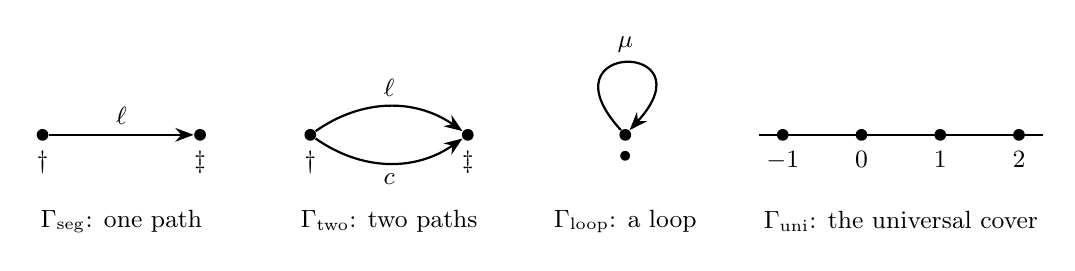
\begin{tikzpicture}[>=Stealth,every node/.style={font=\small}]
\begin{scope}
\node[circle,fill,inner sep=1.5pt,label=below:$\dagger$] (a) at (0,0) {};
\node[circle,fill,inner sep=1.5pt,label=below:$\ddagger$] (b) at (2,0) {};
\draw[->,thick] (a) -- node[above] {$\ell$} (b);
\node[align=center] at (1,-1.1) {$\Gseg$: one path};
\end{scope}
\begin{scope}[xshift=3.4cm]
\node[circle,fill,inner sep=1.5pt,label=below:$\dagger$] (a) at (0,0) {};
\node[circle,fill,inner sep=1.5pt,label=below:$\ddagger$] (b) at (2,0) {};
\draw[->,thick] (a) to[bend left=35] node[above] {$\ell$} (b);
\draw[->,thick] (a) to[bend right=35] node[below] {$c$} (b);
\node[align=center] at (1,-1.1) {$\Gtwo$: two paths};
\end{scope}
\begin{scope}[xshift=6.8cm]
\node[circle,fill,inner sep=1.5pt,label=below:$\bullet$] (a) at (0.6,0) {};
\draw[->,thick] (a) .. controls (-0.5,1.2) and (1.7,1.2) .. node[above] {$\mu$} (a);
\node[align=center] at (0.6,-1.1) {$\Gloop$: a loop};
\end{scope}
\begin{scope}[xshift=9.4cm]
\draw[thick] (-0.3,0) -- (3.3,0);
\foreach \x/\n in {0/-1,1/0,2/1,3/2} {\node[circle,fill,inner sep=1.5pt,label=below:$\n$] at (\x,0) {};}
\node[align=center] at (1.5,-1.1) {$\Guni$: the universal cover};
\end{scope}
\end{tikzpicture}
\end{center}

\begin{definition}[Families]\label{d:fam}\tagR
\known{\cite[\S2]{MO}}
The type of families of ordered real lines over a graph $\Gamma$ is
\[\Fam(\Gamma):=\Sigma\bigl(L:V\to\LL\bigr).\ \Pi(e:E).\ \bigl(L(\mathrm{s}\,e)=L(\mathrm{t}\,e)\bigr).\]
By Proposition~\ref{p:line}\,(i), the path on an edge $e$ is the same thing as an order isomorphism
$e_*:L(\mathrm{s}\,e)\to L(\mathrm{t}\,e)$.
\end{definition}

\begin{definition}[Values]\label{d:sec}\tagR
\known{\cite[\S2]{MO}}
The type of \emph{values} (sections) of a family $F=(L,p)$ is
\[\Sec(F):=\Sigma\bigl(x:\Pi(v:V).\,L(v)\bigr).\ \Pi(e:E).\ \bigl(e_*\,x(\mathrm{s}\,e)=x(\mathrm{t}\,e)\bigr).\]
It consists of a value at each vertex such that the values agree, whichever edge they are transported along.
\end{definition}

\begin{primedremark}{3.3$'$}
$\Fam(\Gamma)$ is equivalent to the type of maps into $\LL$ from the geometric realization of $\Gamma$ (the higher
inductive type with the vertices as points and the edges as paths), and $\Sec(F)$ to the type of dependent functions
over it. The realization of $\Gloop$ is the circle $\mathbb S^1$ \cite[\S2]{MO}, \cite{CCHM}. In this paper we use
Definitions~\ref{d:fam} and~\ref{d:sec} as they stand.
\end{primedremark}

\subsection{Segment: identifying fibres loses no information}
\begin{proposition}\label{p:seg}\tagP\tagR
\known{\cite[\S3.2]{CCHM} (path induction via the contractibility of singletons)}
\begin{enumerate}[label=(\roman*)]
\item The map $\Fam(\Gseg)\to\LL$, $(L,\ell)\mapsto L(\dagger)$, is an equivalence.
\item For a family $F:\Fam(\Gseg)$, the map $\Sec(F)\to L(\dagger)$, $x\mapsto x(\dagger)$, is an equivalence.
\item Hence, for any proposition $P$ on $\Fam(\Gseg)$, $P$ holds for all families if and only if it holds for the
families of the form $(L,L,\refl_L)$.
\end{enumerate}
\end{proposition}
\begin{proof}
(i) $\Fam(\Gseg)\simeq\Sigma(L^\dagger:\LL).\,\Sigma(L^\ddagger:\LL).\,(L^\dagger=L^\ddagger)$, and the inner part is
contractible by Lemma~\ref{l:single}.
(ii) $\Sec(F)\simeq\Sigma(x^\dagger:L^\dagger).\,\Sigma(x^\ddagger:L^\ddagger).\,(\ell_*x^\dagger=x^\ddagger)$, and the
inner part is contractible by Lemma~\ref{l:single}.
(iii) By (i), every family is equal to a family of the form $(L,L,\refl)$; transport $P$ along that equality.
\end{proof}
\leanref{\lean{segment\_section}}
Proposition~\ref{p:seg} says that identifying copies along one path changes the truth of no proposition. In this sense
the simplification of Scholze--Stix (\q{simply identifying identical objects along the identity}~\cite[\S2.1]{SS}, and the \q{obvious} isomorphisms of
\cite[footnote~8]{SS}) and Mochizuki's \q{it is always possible to consider the situation in which one \textbf{deletes} the \textbf{labels} `$\dagger$', `$\ddagger$'}~\cite[Example~2.4.8\,(iv-c)]{Ess} are correct.

\subsection{Two paths make a loop}
\begin{proposition}\label{p:two}\tagP\tagR
\known{\cite[\S2]{MO}, \cite{CCHM}}
The map
\[\Fam(\Gtwo)\longrightarrow\Sigma(L:\LL).\,(L=L),\qquad (L,\ell,c)\longmapsto\bigl(L(\dagger),\ \ell\cdot
c^{-1}\bigr)\]
is an equivalence.
\end{proposition}
\begin{proof}
Rearrange
$\Fam(\Gtwo)\simeq\Sigma(L^\dagger:\LL).\ \Sigma\bigl((L^\ddagger,c):\Sigma(L^\ddagger:\LL).(L^\dagger=L^\ddagger)\bigr).\
(L^\dagger=L^\ddagger)$. By Lemma~\ref{l:single}, $\Sigma(L^\ddagger).(L^\dagger=L^\ddagger)$ contracts to
$(L^\dagger,\refl)$, so the whole is equivalent to $\Sigma(L^\dagger).(L^\dagger=L^\dagger)$. That this contraction
sends the remaining path $\ell$ to $\ell\cdot c^{-1}$ is checked by path induction on $c$, reducing to the case
$c\equiv\refl$.
\end{proof}

\begin{definition}[Monodromy]\label{d:mono}\tagR
\known{\cite[(LbEx1)]{R18}, \cite[\S2.2]{SS}}
The \emph{monodromy} of a family $F=(L,\ell,c):\Fam(\Gtwo)$ is the automorphism
$c_*^{-1}\circ\ell_*\in\Aut(L(\dagger))$, and its scale is written $m(F):=\sigma\bigl(c_*^{-1}\circ\ell_*\bigr)\in\Rp$.
\end{definition}

\begin{proposition}[The monodromy is a complete invariant]\label{p:complete}\tagP\tagR
\known{\cite[\S2]{MO} (families over a delooping and group actions)}
\begin{enumerate}[label=(\roman*)]
\item If $F=F'$ (an identification of families), then $m(F)=m(F')$. Concretely, re-identifying by order isomorphisms
$\varphi:L(\dagger)\cong L'(\dagger)$ and $\psi:L(\ddagger)\cong L'(\ddagger)$, so that $\ell'=\psi\ell\varphi^{-1}$ and
$c'=\psi c\varphi^{-1}$, does not change $m$.
\item The scale gives an equivalence $\trunc{\Fam(\Gtwo)}_0\simeq\Rp$. That is, two families are equal (as a
proposition) if and only if the scales of their monodromies are equal.
\end{enumerate}
\end{proposition}
\begin{proof}
(i) $m$ is a function on $\Fam(\Gtwo)$, so it is preserved along paths. Concretely,
$c'^{-1}\ell'=\varphi\,(c^{-1}\ell)\,\varphi^{-1}$, and by Proposition~\ref{p:line}\,(iii) the scale does not change
under conjugation.

(ii) Surjectivity: for $r\in\Rp$, the family $(\R,\R,\,x\mapsto rx,\ \id)$ has scale $r$. Injectivity: by
Proposition~\ref{p:two} it suffices to consider $(L_1,\mu_1)$ and $(L_2,\mu_2)$ (with $\mu_i:L_i=L_i$) such that
$\sigma(\mu_1)=\sigma(\mu_2)$. By Proposition~\ref{p:line}\,(iv) we may take (as a proposition) a path $q:L_1=L_2$. The
transport of $\mu_1$ along the family $L\mapsto(L=L)$ is $q^{-1}\cdot\mu_1\cdot q$ (the transport formula in identity
types~\cite{MO}), and its scale equals $\sigma(\mu_1)$ (Proposition~\ref{p:line}\,(iii)). Since $\sigma_{L_2}$ is
injective, $q^{-1}\mu_1q=\mu_2$, and hence $(L_1,\mu_1)=(L_2,\mu_2)$.
\end{proof}
\leanref{\lean{monodromy\_relabel}, \lean{route\_factor}}
Propositions~\ref{p:two} and~\ref{p:complete} say that as soon as a second path is brought in, a family over the two
stages becomes a family over a loop, and that its monodromy does not disappear however one re-identifies. What the
identification along the first path (Proposition~\ref{p:seg}) removes is only the distinction of the vertex $\ddagger$;
the discrepancy between the two paths remains.

\subsection{Values on the loop are fixed points}
\begin{proposition}\label{p:fixed}\tagP\tagR
\known{\cite[\S2]{MO}, \cite[(LbEx1)]{R18}}
Let $m$ be the scale of the monodromy of a family $F:\Fam(\Gtwo)$. Then
\[\Sec(F)\ \simeq\ \{\,x\in L(\dagger)\mid m\,x=x\,\}.\]
In particular, if $m\ne1$ the only value is zero, and if $m=1$ then $\Sec(F)\simeq L(\dagger)$. Moreover, ``every $x$
extends to a value'' is equivalent to $m=1$.
\end{proposition}
\begin{proof}
$\Sec(F)\simeq\Sigma(x^\dagger).\,\Sigma(x^\ddagger).\,(\ell_*x^\dagger=x^\ddagger)\times(c_*x^\dagger=x^\ddagger)$.
Contracting $x^\ddagger$ with the second equation gives
$\Sigma(x^\dagger).\,(\ell_*x^\dagger=c_*x^\dagger)\simeq\Sigma(x^\dagger).\,(c_*^{-1}\ell_*\,x^\dagger=x^\dagger)$, and
by Proposition~\ref{p:line}\,(ii) the condition is $m x^\dagger=x^\dagger$. If $m\ne1$, then $(m-1)x=0$ gives $x=0$.
\end{proof}
\leanref{\lean{loopSection\_iff\_fixed}, \lean{loopSection\_iff\_zero}, \lean{all\_values\_consistent\_iff}}

\subsection{The universal cover}
\begin{proposition}\label{p:uni}\tagP\tagR
\known{\cite[(LbEx1)]{R18} (universal cover)}
For $L:\LL$ and $g\in\Aut(L)$ (of scale $m$), build a family over $\Guni$ by putting $L$ at every vertex and $g$ on every
edge. Its type of values is equivalent to $L$, via $x\mapsto(g^nx)_{n\in\Z}$. In particular, values exist for
every~$m$.
\end{proposition}
\begin{proof}
A value is a sequence $(x_n)_{n\in\Z}$ with $g\,x_n=x_{n+1}$, and it is determined uniquely by $x_0$ as $x_n=g^nx_0$
(with $g^{-1}$ for negative $n$).
\end{proof}
\leanref{\lean{uni\_edge}}

\subsection{Mochizuki's three graphs}
\srcquote{\q{One considers the \emph{(`line segment') graph} $\Gamma_{\mathrm{seg}}$ \dots{} given by \emph{two vertices}
joined via a \emph{single edge}. Write $\Gamma_{\mathrm{loop}}$ for the \emph{(`loop') graph} obtained from
$\Gamma_{\mathrm{seg}}$ by identifying the \emph{two distinct vertices} of $\Gamma_{\mathrm{seg}}$ --- i.e., which may be
thought of as \emph{distinct labels} --- to a \emph{single vertex}. \dots{} situations where some sort of
\textbf{`parallel transport'} or \textbf{`analytic continuation'} along the \textbf{loop} of $\Gamma_{\mathrm{loop}}$ gives
rise to some sort of \textbf{nontrivial monodromy operator}. This sort of nontrivial monodromy may be \textbf{resolved}
\dots{} \emph{by working over $\Gamma_{\mathrm{seg}}$ as opposed to $\Gamma_{\mathrm{loop}}$}. When, moreover, one wishes
to distinguish situations that arise \emph{prior to} and \emph{subsequent to} multiple applications of the monodromy
operator, it is natural to consider the \emph{universal covering} $\Gamma_{\mathrm{uni}}$ \dots{} of
$\Gamma_{\mathrm{loop}}$} \dots\par
\q{one may understand the \textbf{incompatibility} of the \textbf{\boldmath$\Theta$-link} \dots{} with \textbf{arithmetic
degrees} \dots{} as a sort of \textbf{nontrivial monodromy} around the \textbf{loop} \dots{} that arises as soon as one
\emph{identifies} the \emph{domain} and \emph{codomain} of the $\Theta$-link --- an incompatibility \dots{} that is in fact
\textbf{avoided} in IUTch \dots{} precisely by \textbf{distinguishing} \emph{the (ring structures in the) domain and
codomain of the $\Theta$-link}, i.e., by working with `$\Gamma_{\mathrm{seg}}$', and then applying the \textbf{multiradial
algorithms} of IUTch to obtain an alternative way to \textbf{compute this nontrivial monodromy}}}{\cite[\S14,
(LbEx1)]{R18}}

\tagH\ The propositions of this paper turn this explanation into types as it stands. On $\Gseg$ the values are
unconstrained (Proposition~\ref{p:seg}). On $\Gloop$ the values are restricted to the fixed points of the monodromy
(Proposition~\ref{p:fixed}). On $\Guni$ there are values for every monodromy (Proposition~\ref{p:uni}). However, as
Proposition~\ref{p:two} shows, identifying \q{the \emph{domain} and \emph{codomain} of the $\Theta$-link} needs a second
path. In our reading, the multiradial algorithm
provides a second path $c$, different from the $\Theta$-link. Therefore, as soon as one compares by two paths, the
family becomes a family over a loop (Proposition~\ref{p:two}). The monodromy is an invariant whose value is determined
by what Mochizuki calls \q{an alternative way to \textbf{compute this nontrivial monodromy}}, and it does not disappear by
re-identification (Proposition~\ref{p:complete}). That the incompatibility is \q{\textbf{avoided}} in IUTch can be read
as meaning that single-valuedness on the loop (Proposition~\ref{p:fixed}) is not required. The question that then remains is treated in Section~\ref{s:step}.

\section{Possible images, logical AND and OR, and descent}\label{s:poss}
\begin{definition}[Possible images]\label{d:poss}\tagR
\known{\cite[Cor.~3.12]{IUT3} (possible images)}
For a map $\pi:X\to Y$ and a family of subsets $\Phi:X\to\mathcal P(Z)$, the family of \emph{possible images} is
\[\Psi_\pi\Phi(y):=\{\,z\mid\exists(x:X).\ \pi(x)=y\ \wedge\ z\in\Phi(x)\,\}.\]
Here $X$ is the data with labels (choices of indeterminacies), $Y$ the data with the labels forgotten, and $\pi$ the
forgetting.
\end{definition}

\begin{proposition}[Universality]\label{p:univ}\tagP\tagR
\known{\cite{MR} (existential quantification is left adjoint to substitution)}
For $\Psi:Y\to\mathcal P(Z)$,
\[\bigl(\forall y.\ \Psi_\pi\Phi(y)\subseteq\Psi(y)\bigr)\iff\bigl(\forall x.\ \Phi(x)\subseteq\Psi(\pi x)\bigr).\]
That is, the union of possible images is the smallest label-independent family that contains all the labelled images.
\end{proposition}
\begin{proof}
($\Rightarrow$) If $z\in\Phi(x)$, then $z\in\Psi_\pi\Phi(\pi x)\subseteq\Psi(\pi x)$. ($\Leftarrow$) We are to show
$z\in\Psi(y)$ (a proposition) from $z\in\Psi_\pi\Phi(y)$, so we may extract from $\exists$ an $x$ with $\pi x=y$ and
$z\in\Phi(x)$. Then $z\in\Psi(\pi x)$, and transporting along $\pi x=y$ gives $z\in\Psi(y)$.
\end{proof}
\leanref{\lean{possibleImages\_universal} (uses no axioms)}

\begin{definition}[Labelled pairs and unlabelled sets]\label{d:pair}\tagR
\known{\cite[Example~2.4.8\,(iv-c)]{Ess}}
For a family of two paths $F=(L,\ell,c)$ and $x\in L(\dagger)$, define the \emph{labelled pair}
$\lambda_x:\{\mathrm{link},\mathrm{core}\}\to L(\ddagger)$ by $\lambda_x(\mathrm{link})=\ell_*x$ and
$\lambda_x(\mathrm{core})=c_*x$, and the \emph{unlabelled set} $U_x:=\{w\mid\exists r.\ \lambda_x(r)=w\}$. The former
corresponds to ``along both paths it is attached in this way'' ($\wedge$), the latter to ``along one of the paths it is
attached in this way'' ($\vee$).
\end{definition}

\begin{proposition}\label{p:andor}\tagP\tagR
\known{\cite[Example~2.4.8\,(iv-c)]{Ess}}
\begin{enumerate}[label=(\roman*)]
\item $U_x$ does not change if the roles of the two paths are interchanged.
\item If $m(F)\ne1$ and $x\ne0$, then $\lambda_x(\mathrm{link})\ne\lambda_x(\mathrm{core})$.
\item There is no function that, looking only at the unlabelled set, returns the value attached on the side of the
$\Theta$-link. That is, there is no $G:\mathcal P(\R)\to\R$ with $G(U_x)=\ell_*x$ for all families and all~$x$.
\end{enumerate}
\end{proposition}
\begin{proof}
(i) The image of a function on a two-point set does not change when the swap is composed in front. (ii)
Proposition~\ref{p:fixed}. (iii) Compare, at $x=1$, the family $(\R,\R,\,x\mapsto2x,\ \id)$ and the family obtained by
interchanging its two paths. By (i) they have the same $U_1=\{1,2\}$, but the values on the side of the $\Theta$-link
are $2$ and $1$, which differ.
\end{proof}
\leanref{\lean{unlabelled\_swap}, \lean{labelled\_distinct}, \lean{link\_value\_not\_recoverable}}

\srcquote{\q{it is always possible to consider the situation in which one \textbf{deletes} the \textbf{labels}
`$\dagger$', `$\ddagger$', but only at the expense of \textbf{sacrificing} these \textbf{crucial logical AND} properties
(iv-a), (iv-b), i.e., at the expense of agreeing to work under the assumption that the `glued data' is the data
associated to `$\dagger$' \textbf{OR} the data associated to `$\ddagger$', but \emph{not necessarily both
simultaneously}.}}{\cite[Example~2.4.8\,(iv-c)]{Ess}}

\tagH\ After the copies are identified, glued data appear as two paths into the same container.
Proposition~\ref{p:andor} says that when the labels are deleted, what remains is only the set $U_x$ ($\vee$), and the
pair $\lambda_x$ ($\wedge$) does not come back.

\begin{definition}[Descent]\label{d:descent}\tagR
\known{\cite[\S3.9]{Ess}}
For a map $p:A\to B$ and a construction $\Phi:A\to C$, we say that $\Phi$ \emph{descends} to $B$ if there is
$\Psi:B\to C$ with $\Phi\circ\id=\Psi\circ p$ (as a pointwise identification). When $B$ is a truncation or a quotient of
$A$ and $C$ is a set, descending is equivalent to $\Phi$ being unchanged by the identifications of~$A$.
\end{definition}

\srcquote{Descent (\S3.9): \q{a \emph{functorial algorithm} $\Phi$ in the \emph{original data} \textbf{descends} to a
\emph{functorial algorithm} $\Psi$ in the \emph{underlying data} if there exists a functorial isomorphism
\[\Phi\stackrel{\sim}{\to}\Psi|_{\textit{original data}}\]
between $\Phi$ and the \emph{restriction} of $\Psi$} \dots. (ExtInd2) (\S3.6) \q{may be thought of as a sort of actual
\textbf{descent operation}, i.e., from data that \emph{depends} on the specification of a member of some collection of
\emph{distinct labels} to data that is \emph{independent} of such a label specification}. (DltLb) (\S3.11): the distinct
labels are to be deleted \q{\textbf{not} via the \emph{naive, simple-minded} approach \dots, but rather via the
\emph{indirect approach} of applying \textbf{descent operations}}. (FrgInv) (\S3.11): \q{the operation of
\textbf{forgetting} \dots{} can in fact, if one allows for suitable \textbf{indeterminacies}, be
\textbf{inverted}.}}{\cite[\S3.9, \S3.6, \S3.11]{Ess}}

\tagH\ Definition~\ref{d:descent} is the definition of~\cite[\S3.9]{Ess} itself. If a label-dependent construction is
identified naively, one ends up requiring values on the loop (Proposition~\ref{p:fixed}). In descent, the values are
enlarged to the set of possible images (Proposition~\ref{p:univ}), so this does not happen. However, the result
changes according to along which identifications one descends (over the orbits of which groupoid the union is taken).
This is the subject of Section~\ref{s:step}. With the components of tensor packets, the label permutations of (Ind1)
give a further, finite groupoid; Part~II of~\cite{UE} computes the union over it in two readings and shows, in a model,
that in either reading Corollary~3.12 together with the upper bound of IV implies the height bound.

\section{Step (xi): two paths and 2-cells}\label{s:step}

\subsection{The model}
\srcquote{Corollary~3.12: write $-|\log(\Th)|\in\R\cup\{+\infty\}$ for the procession-normalized mono-analytic
log-volume of the holomorphic hull of the union of the possible images of a $\Theta$-pilot object in the multiradial
representation of Theorem~3.11, which is regarded as subject to the indeterminacies (Ind1), (Ind2), (Ind3); and write
$-|\log(\qq)|\in\R$ for the procession-normalized mono-analytic log-volume of the image of a $q$-pilot object, which is not
regarded as subject to these indeterminacies. Here $|\log(\qq)|>0$. Then \q{it holds that
$-|\log(\underline{\underline{\Theta}})|\in\mathbb{R}$, and
$-|\log(\underline{\underline{\Theta}})|\geq-|\log(\underline{\underline{q}})|$}.}{\cite[Cor.~3.12]{IUT3}}

\begin{setup}[A model of the comparison of Step~(xi)]\label{setup}\tagR
\known{\cite[\S2.1.4, \S2.2]{SS}, \cite[\S7.1, \S10.2]{LANA}}
Consider the following data.
\begin{enumerate}[label=(\alph*)]
\item Two ordered real lines $L^\dagger,L^\ddagger:\LL$: the containers of the values that log-volumes and degrees take
on the two sides of the $\Theta$-link (the $\R_{\odot,\Theta}$, $\R_{\odot,q}$ of Scholze--Stix, the $\R^{\mathrm{val}}$,
$\R^{\mathrm{ss}}$ of LANA).
\item Two paths $\ell,c:L^\dagger=L^\ddagger$. Here $\ell$ is the identification induced by the $\Theta$-link (sending
the abstract $\Theta$-pilot to the abstract $q$-pilot), and $c$ is the standard identification via the shared data (the
coric data).
\item $b\in L^\dagger$ is the log-volume of the $\Theta$-pilot, and $a\in L^\ddagger$ the log-volume of the $q$-pilot.
IPL: $\ell_*b=a$.
\item The coordinate of $L^\ddagger$ is chosen so that $c$ is the identity (coric coordinates). Put $Q:=|\log(\qq)|>0$
and $a=-Q$. If $m:=\sigma(c_*^{-1}\ell_*)$ is the scale of the monodromy, then $c_*b=-Q/m$.
\item A blurring $E\ge0$: the value of the holomorphic hull of the union of the possible images of the $\Theta$-pilot,
computed through $c$, is $-|\log(\Th)|:=c_*b+E$ (the excess from taking the holomorphic hull of the union of
Proposition~\ref{p:univ}).
\item Corollary~3.12 (model): $a\le c_*b+E$.
\end{enumerate}
\end{setup}

\begin{quote}\small\tagX\ Scholze--Stix write that \q{There is one consistent choice of isomorphisms given by using the
natural isomorphisms $\mathbb{R}_{\odot,\Theta}\cong\mathbb{R}_{\odot,q}\cong\mathbb{R}$}. With these isomorphisms,
however, the abstract $\Theta$-pilot object does not encode the arithmetic degree, so scalars $j^2$ are to be introduced
on the left ($\Theta$-) part of the diagram, and \q{it is clear that this will result in the whole diagram having
monodromy $j^2$, i.e., being inconsistent} \cite[\S2.2]{SS}. LANA reproduces the hexagon of Scholze--Stix, confirms that
it does not commute, and reads it as follows: \q{The composition $\mathbb{R}_{\odot,\Theta}\to\mathbb{R}_\Theta$ scales by
a factor of $\frac{1}{\ell^{\divideontimes}}(1^2+2^2+\cdots+(\ell^{\divideontimes})^2)$ while the composition
$\mathbb{R}_{\odot,q}\to\mathbb{R}_q$ scales by a factor of 1} \cite[\S10.2]{LANA}.\end{quote}

In this reading $m=\bigl(\frac{1}{l^\ast}\sum_{j=1}^{l^\ast}j^2\bigr)^{-1}$, where $l^\ast=(l-1)/2$ (written
$\ell^{\divideontimes}$ in~\cite{SS,LANA}), and $0<m<1$ if $l^\ast\ge2$. The
theorems below use only $0<m<1$ and do not depend on the value of~$m$.

\begin{primedremark}{5.1$'$ (What lies outside the model)}
How the theory constructs $E$ (the multiradial algorithm of Theorem~3.11) and how IV estimates $E$ from above
(IV, Theorem~1.10) lie outside the model. The latter is used only as the assumption $E\le C$.
\end{primedremark}

\subsection{There is no strict 2-cell}
\begin{theorem}\label{t:strict}\tagP\tagR
\known{\cite[(AD), (IUAD)]{R18}, \cite[\S2.2]{SS}}
In Setup~\ref{setup}, $\ell_*b=c_*b$ holds only if $m=1$ or $b=0$. Hence, under $0<m<1$, $\ell_*b\ne c_*b$: the two paths
do not agree on the $\Theta$-pilot, and there is no strict 2-cell joining the two paths.
\end{theorem}
\begin{proof}
Apply Proposition~\ref{p:fixed} to $x=b$; note that $b=-Q/m\ne0$.
\end{proof}
\leanref{\lean{Step.no\_strict\_cell}}

\srcquote{(AD) \q{The correspondence that appears in the \textbf{\boldmath$\Theta$-link}
\[\{\underline{\underline{q}}^{j^2}\}\quad\mapsto\quad\underline{\underline{q}}\]
(where $j=1,\ldots,l^{\divideontimes}$) is, when considered within/relative to a \textbf{single hol.\ str.}, i.e., a
\textbf{single ring/scheme theory}, manifestly \textbf{incompatible/inconsistent} with computing \textbf{arithmetic
degrees}, unless one considers arithmetic degrees up to the \textbf{indeterminacy} \emph{given by possible multiplication
by factors `$j^2$'} (where $j=1,\ldots,l^{\divideontimes}$) --- an indeterminacy which then renders the computation
\emph{meaningless}.}\par
(IUAD) \q{There is \textbf{absolutely no dispute} whatsoever (between SS and HM) with respect to the validity of the
assertion (AD).}}{\cite[\S12, (AD), (IUAD)]{R18}}

\tagH\ Theorem~\ref{t:strict} and Proposition~\ref{p:fixed} are the type-theoretic form of the first half of (AD)
(incompatibility), and Theorem~\ref{t:loop} is that of the second half (introducing the indeterminacy renders the
computation meaningless). As Mochizuki says, there is no dispute here.

\subsection{Corollary 3.12 is a lax 2-cell}
\begin{theorem}\label{t:lax}\tagP\tagR
\known{\cite[\S2.2]{SS} (the blurring must be by a factor of at least $O(l^2)$), \cite[\S0.2]{LANA} (the \q{wall})}
In Setup~\ref{setup} the following are equivalent.
\begin{enumerate}[label=(\roman*)]
\item Corollary~3.12 (model): $a\le c_*b+E$.
\item A lax 2-cell: $\ell_*b\le c_*b+E$. That is, the value transported along the path of the $\Theta$-link does not
exceed the value transported along the path of the shared data, widened by the blurring.
\item $\bigl(\tfrac1m-1\bigr)Q\le E$.
\end{enumerate}
\end{theorem}
\begin{proof}
(i)$\Leftrightarrow$(ii) by IPL, $\ell_*b=a$. (ii)$\Leftrightarrow$(iii): since $\ell_*b=-Q$ and $c_*b=-Q/m$, we have
$-Q\le-Q/m+E\iff Q/m-Q\le E\iff(1/m-1)Q\le E$.
\end{proof}
\leanref{\lean{Step.cor312\_iff\_lax}, \lean{Step.cor312\_iff\_blur}}

\begin{corollary}\label{c:height}\tagP\tagR
\known{\cite[Thm.~1.10]{IUT4}, \cite[Introduction]{Alien}}
In Setup~\ref{setup}, if $E\le C$, then Corollary~3.12 (model) implies $Q\le C/(1/m-1)$. If $E=0$ (no blurring), then
Corollary~3.12 (model) does not hold.
\end{corollary}
\begin{proof}
From Theorem~\ref{t:lax}\,(iii) and $1/m-1>0$. If $E=0$, the left-hand side of (iii) is positive, so (iii) fails.
\end{proof}
\leanref{\lean{Step.height\_bound}, \lean{Step.cor312\_needs\_blur}}
Theorem~\ref{t:lax} is the precise form of Scholze--Stix's statement that \q{the blurring must be by a factor of at least $\mathrm{O}(\ell^2)$}~\cite[\S2.2]{SS}. In
multiplicative terms, the absolute value of the hull must be at most $m$ times that of the image, that is, it must have
shrunk by the factor $1/m=\frac1{l^\ast}\sum j^2=O(l^2)$. Corollary~\ref{c:height} shows that whether this is
``useless'' or ``the content of the theory'' hinges exactly on $E\le C$, that is, on the height bound itself.
Neither evaluation follows from logic alone.

\begin{primedremark}{5.4$'$ (A consistent identification is not a necessary condition)}
\tagH\ The comparison of Theorem~\ref{t:lax} requires no value on the loop (Proposition~\ref{p:fixed}); it requires
only one inequality. Hence the general principle ``a meaningful comparison requires a consistent identification of the
copies of the real numbers'' does not hold. What remains is only the size of the blurring.
\end{primedremark}

\subsection{A hull along the loop says nothing}
\begin{theorem}\label{t:loop}\tagP\tagR
\known{\cite[Remark~3.11.1\,(vii),\,(viii)]{IUT3}}
In Setup~\ref{setup}, suppose that a value $H\in\R$ of the hull (in coric coordinates) bounds from above the whole orbit
of the $\Theta$-pilot under the monodromy, that is, $m^n\,c_*b\le H$ for all $n\in\N$. Then $H\ge0\ge a$. Hence
Corollary~3.12 (model) holds whatever $Q$ is, and says nothing about~$Q$.
\end{theorem}
\begin{proof}
We have $c_*b<0$. Suppose $H<0$. By the Archimedean property there is an $n$ with $m^n<(-H)/(-c_*b)$, and then
$m^nc_*b>H$, a contradiction.
\end{proof}
\leanref{\lean{orbit\_hull\_nonneg}, \lean{Step.loop\_hull\_trivial}}

\srcquote{\q{one is led [at least in the absence of more sophisticated machinery!] to regard
`$\underline{\underline{q}}$' as being \textbf{only well-defined up to possible confusion with
`\boldmath$\underline{\underline{q}}^{\lambda^n}$'}, for some indeterminate $n\in\mathbb{Z}$. That is to say, in summary,
this approach gives rise to a sort of \textbf{`uninteresting/trivial multiradial representation} of
`$\underline{\underline{q}}^{\lambda}$' via}
\[\text{``}\{\underline{\underline{q}}^{\lambda^n}\}_{n\in\mathbb{Z}}\text{''}\]
\dots\par
\q{this `trivial multiradial representation' is \textbf{useless} from the point of view of applications such as the
log-volume estimates given in Corollary 3.12 below \dots{} for the following reasons: This \textbf{`trivial multiradial
representation \boldmath$\{\underline{\underline{q}}^{\lambda^n}\}_{n\in\mathbb{Z}}$'} is obtained by
\textperiodcentered\ allowing for \textbf{indeterminacies} in the \textbf{value group} portion [i.e.,
`$\underline{\underline{q}}^{\mathbb{Z}}$'] of the data under consideration, \dots}\par
\q{By contrast, the \emph{log-volume estimates} of Corollary 3.12 below rely, in an essential way, on the fact that in the
\textbf{multiradial construction algorithm} of Theorem 3.11: \textperiodcentered\ the \textbf{value group} portions of the
data under consideration \dots{} are held \textbf{rigid} [i.e., are not subject to indeterminacies],
\textperiodcentered\ while the \textbf{unit group} portions of the data under consideration \dots{} are subject to the
\textbf{indeterminacies} (Ind1), (Ind2), (Ind3); \dots}}{\cite[Remark~3.11.1\,(vii),\,(viii)]{IUT3}}

\tagH\ Theorem~\ref{t:loop} is the type-theoretic form, at the level of log-volumes, of this \q{trivial multiradial representation}, and also
that of the \q{empty inequality} of Scholze--Stix~\cite[\S2.2]{SS}. Here, too, the two sides agree.

\subsection{Qualitative properties do not decide the 2-cell}
\begin{definition}[IPL, SHE and APT in the model]\label{d:package}\tagR
\known{\cite[Remark~3.11.1\,(iii),\,(iv)]{IUT3}}
For the data of Setup~\ref{setup}:
\begin{itemize}
\item IPL: $\ell_*b=a$ (the $\Theta$-link carries the $\Theta$-pilot to the $q$-pilot).
\item SHE: the value of the hull is a function of the shared data; that is, there is an $f$ with
$-|\log(\Th)|=f(c_*b)$.
\item APT: the construction commutes with re-coordinatizations of the shared data; that is, $\varphi(c_*b)=c_*(\varphi\,b)$
for every order isomorphism~$\varphi$.
\end{itemize}
\end{definition}

\srcquote{IPL: the output is constructed so as to be linked, via full poly-isomorphisms of prime-strips, to the
input prime-strip. SHE: the construction of the output, as well as the output itself, is expressed in \q{terms that are
\textbf{simultaneously} valid/executable/well-defined} relative to the arithmetic holomorphic structures in both the
domain and the codomain of the $\Theta$-link. APT: \q{This parallel transport mechanism does \textbf{not} consist of a
simple instance of transport of \emph{some set-theoretic region} \dots{} \emph{via some set-theoretic function}. Rather, it
consists of a \textbf{construction algorithm} \dots} In Step~(xi), \q{we shall \emph{only be concerned} with
\textbf{qualitative logical aspects/consequences}} of this construction algorithm.}{\cite[Remark~3.11.1\,(iii),\,(iv),
and Step~(xi-b) of the proof of Cor.~3.12]{IUT3}}

\begin{theorem}\label{t:package}\tagP\tagR
\known{\cite{Hi}}
For any $0<m<1$ and $Q>0$ there are two data $K_1,K_2$ as in Setup~\ref{setup} (with this $m$ and $Q$), both satisfying
IPL, SHE and APT, such that Corollary~3.12 (model) fails in $K_1$ and holds in~$K_2$.
\end{theorem}
\begin{proof}
In $K_1$ take $E=0$, and in $K_2$ take $E=(1/m-1)Q$. IPL holds by construction. SHE holds with $f(t)=t+E$. APT holds
because $c$ is the identity in coric coordinates. Whether Corollary~3.12 holds follows from Corollary~\ref{c:height} and
Theorem~\ref{t:lax}.
\end{proof}
\leanref{\lean{package\_holds}, \lean{package\_does\_not\_decide}}

\tagH\ In homotopy type theory, every construction defined on the type of the shared data is automatically
transported along paths (APT) and factors through the shared data (SHE). IPL is the existence of one path. That is, all
three properties are one-dimensional data (paths and functoriality) and decide nothing about 2-cells between the two
paths. Theorem~\ref{t:package} is the quantitative form of this. The same conclusion has been proved by Higuchi, for the
passage from Step~(xi-e) to Step~(xi-f), in a different formalization~\cite{Hi}.

\srcquote{The \emph{``possible images''} output by the multiradial algorithm \q{\textbf{cannot} be
\textbf{directly compared} [i.e., at least in any \emph{a priori} sense] to the \emph{objects} in the \emph{local} and
\emph{global Frobenioids} that appear in the \emph{codomain}
$\mathcal{F}^{\Vdash\blacktriangleright\times\boldsymbol{\mu}}$-\emph{prime-strip} of the
$\Theta^{\times\boldsymbol{\mu}}_{\mathrm{LGP}}$-link \dots{} determined by the \textbf{arithmetic line bundle} that gives
rise to the \textbf{\boldmath$q$-pilot object}}. This obstruction is eliminated by the $\mathcal{O}^\times$-indeterminacies
acting on tensor packets of log-shells (Ob1), by the passage from arbitrary regions to hulls (Ob2), by the passage from
arithmetic vector bundles to arithmetic line bundles by forming determinants (Ob3), and so on; the result \q{may be
\textbf{compared}, in a meaningful way, to the objects determined by the \emph{arithmetic line bundle} that gives rise to
the \textbf{\boldmath$q$-pilot object}}.}{\cite[Remark~3.9.5\,(vii)]{IUT3}; see also \cite[Remark~3.11.1\,(iv)]{IUT3}}

\begin{remark}[Being comparable, and the comparison holding]\label{r:comparable}\tagH\ 
The procedure of Remark~3.9.5\,(vii) carries the hull of the possible images to an object of the same type as the
$q$-pilot, and so makes the comparison ``well-typed''. In the language of this paper, it corresponds to the guarantee
that the value in (e) of Setup~\ref{setup} lives in $L^\ddagger$ and that the inequality of (f) can be written down.
That the inequality holds, that is, the 2-cell, is a separate assertion. Moreover, SHE in Definition~\ref{d:package} is
the weak reading (being a function of the shared data). If SHE is read in the strong sense that ``the output is directly
comparable with the structure of the codomain and contains the $q$-pilot'', then SHE itself asserts the 2-cell and, by
Theorem~\ref{t:lax}, contains content equivalent to the height bound. In either reading, the 2-cell does not come from
logic alone.
\end{remark}

\subsection{The two readings in the same form}\label{ss:readings}
\begin{quote}\small\tagX\ In LANA's understanding, the inequality of Corollary~3.12 \q{is not obtained by comparing the
volumes of two pilots situated on the two sides of the $\Theta$-link} but within the arithmetic holomorphic structure on
one side of it, and the proof \q{rests on the comparison (9-1)} between the isomorphism $\eta^q$ obtained from the
$q$-pilot and the isomorphism $\eta^{\mathrm{anab}}_S$ obtained by anabelian and Kummer-theoretic procedures (both from
$\mathbb{R}^{\mathrm{val}}$ to $\mathbb{R}^{\mathrm{ss}}$), namely $\eta^q=\eta^{\mathrm{anab}}_S$ for a suitable $S$.
Accordingly, \q{the non-commutativity of the diagram in Figure 7 does not, by itself, establish a defect in the intended
proof strategy} (Figure~7 is the hexagon of Scholze--Stix). On the other hand, LANA records that \q{the problem
concentrates on the proposition of whether, after taking 1st, 2nd, and 3rd indeterminacies into account, a certain
diagram is commutative, or a certain isomorphism can be said to be the identity}.\par\nopagebreak\hfill{\footnotesize
\cite[\S10.2, \S10.3, \S9.2, \S0.2]{LANA}}\end{quote}

\tagH\ The hexagon of Scholze--Stix compares two paths joining the two sides of the $\Theta$-link. LANA's (9-1)
compares, on one side of the $\Theta$-link, two paths $\eta^q$, $\eta^{\anab}$ from $\R^{\mathrm{val}}$ to
$\R^{\mathrm{ss}}$. Both have the form of asserting a 2-cell between two paths, modulo indeterminacies (the choice
of~$S$). The propositions of Sections~\ref{s:fam} and~\ref{s:step} apply as they stand if the paths $(\ell,c)$ are read
as $(\eta^q,\eta^{\anab})$ and the blurring as the orbit of~$S$. Homotopy type theory does not decide which diagram the
proof goes through. What it does decide is that, in either reading, what remains is one 2-cell.

\section{Overview: the vocabularies of the parties and the propositions of this paper}\label{s:overview}
Legend: \tagS\ what the source says; \tagX\ a claim of another author; the columns ``In homotopy type theory'' and
``This paper'' give the correspondence of this paper (a reading, \tagH). The last column lists the propositions and
theorems that apply under that reading.

{\footnotesize
\begin{longtable}{@{}>{\raggedright\arraybackslash}p{4.2cm}>{\raggedright\arraybackslash}p{3.1cm}>{\raggedright\arraybackslash}p{4.3cm}>{\raggedright\arraybackslash}p{2.5cm}@{}}
\toprule
Vocabulary & Source & In homotopy type theory & This paper\\
\midrule
\endhead
The simplification that identifies isomorphic copies; \q{obvious} isomorphisms & \tagX\ \cite[\S2.1, footnote~8]{SS}
& Identification of fibres along one path & Prop.~\ref{p:seg}\\
Deleting the labels is always possible & \tagS\ \cite[Ex.~2.4.8\,(iv-c)]{Ess} & The same & Prop.~\ref{p:seg}\\
Objection to the use of labels (T5); deleting labels amounts to identification or confusion (SSDLFs) & \tagS\
\cite[(T5) of \S4, (SSDLFs)]{R18} & Identification of vertices (with a second path, a loop) &
Props.~\ref{p:two}, \ref{p:complete}\\
$\Gseg$, $\Gloop$, $\Guni$, monodromy & \tagS\ \cite[(LbEx1)]{R18} & Families over a segment, over two paths
($\simeq$ a loop) and over the universal cover & Props.~\ref{p:seg}, \ref{p:fixed}, \ref{p:uni}\\
The monodromy $j^2$; the non-commutativity of the hexagon & \tagX\ \cite[\S2.2]{SS}, \cite[\S10.2]{LANA} & Scale of
the monodromy $m\ne1$; absence of a strict 2-cell & Prop.~\ref{p:complete}, Thm.~\ref{t:strict}\\
(AD), (IUAD): incompatible within one holomorphic structure, meaningless once the indeterminacy is introduced (no
dispute) & \tagS\ \cite{R18} & Values on the loop are fixed points; the hull is trivial & Prop.~\ref{p:fixed},
Thms.~\ref{t:strict}, \ref{t:loop}\\
(LbLV): the labels mark whether the pilot is identified with the log-volume of $q$ or with that of $\{q^{j^2}\}$ &
\tagS\ \cite{R18} & Along which path ($\ell$ or $c$) the containers are identified & Setup~\ref{setup}\,(b)\\
Consistent identification, omission of $j^2$, empty inequality & \tagX\ \cite[\S2.2]{SS} & The hull over the whole
orbit of the loop & Thm.~\ref{t:loop}\\
The blurring must be by a factor of at least $O(l^2)$ & \tagX\ \cite[\S2.2]{SS} & The blurring needed for a lax 2-cell &
Thm.~\ref{t:lax}, Cor.~\ref{c:height}\\
Commutativity of diagrams, identity of isomorphisms, (9-1) & \tagX\ \cite[\S0.2, \S9.2]{LANA} & A 2-cell (modulo
indeterminacies) & Thms.~\ref{t:strict}, \ref{t:lax}, \S\ref{ss:readings}\\
The trivial multiradial representation $\{q^{\lambda^n}\}$ & \tagS\ \cite[Rem.~3.11.1\,(vii)]{IUT3} & The orbit of
the loop & Thm.~\ref{t:loop}\\
The value-group portion is rigid; the unit-group portion is subject to the indeterminacies & \tagS\
\cite[Rem.~3.11.1\,(viii), Step~(xi-b)]{IUT3} & The path of the $\Theta$-link is used once; the blurring is on the
unit-group side & Thm.~\ref{t:lax} (not Thm.~\ref{t:loop})\\
IPL, SHE, APT, HIS & \tagS\ \cite[Rem.~3.11.1\,(iii),\,(iv)]{IUT3} & Paths and functoriality (one-dimensional data) &
Def.~\ref{d:package}, Thm.~\ref{t:package}\\
The holomorphic hull of the union of possible images & \tagS\ \cite[Cor.~3.12]{IUT3} & The sum through truncation
($\exists$) and its excess & Prop.~\ref{p:univ}, Setup~\ref{setup}\,(e)\\
Descent, (ExtInd2), (DltLb) & \tagS\ \cite[\S3.9, \S3.6, \S3.11]{Ess} & Factorization through a quotient or a
truncation & Def.~\ref{d:descent}, Prop.~\ref{p:univ}\\
Logical AND $\wedge$ and logical OR $\vee$ & \tagS\ \cite[Ex.~2.4.8\,(iv-c)]{Ess} & The labelled pair and the unlabelled
set & Prop.~\ref{p:andor}\\
(FrgInv): forgetting can be reversed if indeterminacies are allowed & \tagS\ \cite[\S3.11]{Ess} & Recovery up to an
orbit, not to a point & Prop.~\ref{p:univ} (\tagH)\\
A numerical bridge does not follow from a qualitative package & \tagX\ \cite{Hi} & 1-cells do not decide 2-cells &
Thm.~\ref{t:package}\\
(Ind1), (Ind2) are group actions; (Ind3) is a map on power sets & \tagX\ \cite[\S1, \S4.6]{DH} & Automorphisms of the
shared data (a loop), and laxness by inclusion & Setup~\ref{setup}\,(e)\\
Labelled isomorphic copies; arithmetic Teichm\"uller spaces & \tagX\ \cite[\S1]{Jo1}, \cite[\S1]{Jo2} &
Distinguished points over the same shared data & Section~\ref{s:fam} (\tagH)\\
\bottomrule
\end{longtable}
}

\subsection{What is agreed}
The two paths do not agree strictly (Theorem~\ref{t:strict}). If one makes the values single-valued on the loop, the
only value is $0$, and if one takes the hull over the whole orbit of the loop, the inequality says nothing
(Proposition~\ref{p:fixed}, Theorem~\ref{t:loop}). This is the content of (AD) and (IUAD), and, as Mochizuki writes,
there is no dispute about it between Scholze--Stix and Mochizuki. Moreover, identifying copies along one path loses
nothing (Proposition~\ref{p:seg}). This is the content of the simplification of Scholze--Stix, and Mochizuki also
writes that it is always possible to consider situations in which the labels are deleted
\cite[Example~2.4.8\,(iv-c)]{Ess}.

\subsection{What is disputed}
What remains is the single point of whether a lax 2-cell between the two paths holds, that is, whether
$(1/m-1)Q\le E$ holds (Theorem~\ref{t:lax}). Scholze--Stix, looking at the size of the blurring this needs (a factor of
at least $O(l^2)$), regard the inequality as useless. Mochizuki's side holds that the multiradial algorithm provides
this comparison. LANA's (9-1) states the same point as the agreement of two paths on one side. This inequality itself
has the shape of a height bound ($Q\le E/(1/m-1)$) and is not an independent lemma. By Corollary~\ref{c:height},
together with the upper bound $E\le C$ for the blurring in IV, it gives the height bound $Q\le C/(1/m-1)$.

\subsection{What logic alone does not decide}
The properties IPL, SHE and APT (in the sense of Definition~\ref{d:package}) are compatible with any size of the
blurring (Theorem~\ref{t:package}). Hence, if Step~(xi) uses only \q{qualitative logical aspects/consequences} of these properties, then
Corollary~3.12 does not follow from them, and neither does its negation. If Corollary~3.12 holds, then what provides the
2-cell must be something other than these. The candidates are the size of the values that the comparison procedure of
Remark~3.9.5\,(vii) actually provides, or the quantitative content of the algorithm of Theorem~3.11 (the theta
functions and their values). The latter is what Remark~3.11.1\,(iv) calls \q{hidden internal structures (HIS)}, and it is used essentially in the
computation of log-volumes in IUT~IV. Homotopy type theory does not provide this content, but it shows that the dispute
lies only there.

\subsection{Diagrams, equality and paths: LANA's diagrams and identity types}\label{ss:lana}
LANA writes the point in dispute in the language of diagrams: the hexagon of Scholze--Stix (Figure~7 of LANA) does not
commute; what the proof needs is the compatibility (9-1); and the \q{wall} concentrates on the question of whether a
certain diagram commutes or whether a certain isomorphism can be said to be the identity. This paper has written the
same things with the equality of identity types. The companion paper~\cite{UE} writes them with a symbol for indexed
identifications. In this subsection we put the three ways of writing in one table, and state the relation between the
shape of (9-1) and the shape of Corollary~3.12 as Proposition~\ref{p:lana}.

\xquote{\q{The main goal now is to relate these two kinds of isomorphisms: the one arising from $q$ and the one arising from
anabelian methods. Concretely, we wish to show that there exists some suitable $S$ such that}
\[\eta^q=\eta^{\mathrm{anab}}_S.\tag{9-1}\]
\dots\ \q{(9-1) indicates that the starting point $\eta^q$ belongs to an orbit
(an analogue of a Teichm\"uller deformation) generated by the indeterminacies of the formation of
$\eta^{\mathrm{anab}}_S$.}}{\cite[\S9.2, \S9.3]{LANA}}

\xquote{\q{the indeterminacies create ambiguities in the choice of the set $S$ in (9-1). These ambiguities are reflected in the
log-volume calculation for the hull in IUT IV [13]} \dots\ \q{This description also suggests that the indeterminacies must
be carefully managed so as to keep the log-volume of the hull small enough to yield a meaningful inequality.} \dots\ \q{To
reiterate, we concur that the diagram in Figure 7 does not commute, and that repairing it would require a rescaling factor
that is too large to yield a proof of the \textit{abc} conjecture.} \dots\ \q{However, we, the LANA project, do not have a
proof of (9-1) at this time.}}{\cite[\S10.4, \S10.5]{LANA}; [13] is IUT~IV in LANA's list of references}

\tagH\ Since $\LL$ is a 1-type (Proposition~\ref{p:line}\,(iv)), equality splits into three levels.
\begin{itemize}
\item \emph{Equality of values}: $x=y$ inside one line $L$. Since $L$ is a set, this is a proposition.
\item \emph{Identifications}: paths $p:L=L'$. By Proposition~\ref{p:line}\,(i) they are the same as order
isomorphisms, and together they form a set that is an $\Rp$-torsor.
\item \emph{Agreement of identifications}: equality $p=q$ of paths. Since $\LL$ is a 1-type, this too is a
proposition. That a diagram commutes, or that an isomorphism is the identity, is an assertion at this level.
\end{itemize}

{\footnotesize
\begin{longtable}{@{}>{\raggedright\arraybackslash}p{2.3cm}>{\raggedright\arraybackslash}p{4.2cm}>{\raggedright\arraybackslash}p{2.6cm}>{\raggedright\arraybackslash}p{2.9cm}>{\raggedright\arraybackslash}p{2.0cm}@{}}
\toprule
& LANA (diagrams) & \cite{UE} (indexed identifications) & This paper (identity types) & Level\\
\midrule
\endhead
Values & Elements of the real lines $\R^{\mathrm{val}}$, $\R^{\mathrm{ss}}$ (degrees and log-volumes) & A value
$x\in\R_\alpha$ in a container & A point $x:L$ & Proposition (equality in a set)\\
Identifications & Isomorphisms of based real vector spaces ($\eta^q$, $\eta^{\anab}_S$, the arrows of Figure~7) & The
index $f$ and $x\approx_f y$ & A path $p:L=L'$ & Set (an $\Rp$-torsor)\\
Agreement of identifications & Commutativity of diagrams; an isomorphism being the identity; the equality of (9-1) &
Composites of indices agree (monodromy $1$ around a loop) & Equality $p=q$ of paths (a strict 2-cell) &
Proposition\\
Agreement modulo indeterminacies & (9-1) for a suitable $S$: $\eta^q$ lies in the orbit generated by the
indeterminacies & A set $S$ of indices and $\approx_S$ & $\exists(g\in G).\ \varphi=g\cdot\psi$
(Prop.~\ref{p:lana}\,(a)) & Existence ($(-1)$-truncation)\\
Comparison up to blurring & The computation of log-volumes of hulls (\S10.4) & $\le_E$ & A lax 2-cell
$\ell_*b\le c_*b+E$ (Thm.~\ref{t:lax}) & Inequality of values\\
\bottomrule
\end{longtable}
}

\begin{proposition}[A strict 2-cell modulo indeterminacies, and a lax 2-cell]\label{p:lana}\tagP\tagR
\known{\cite[\S9.2, \S9.3]{LANA} ((9-1)), \cite[\S2.2]{SS}, Theorem~\ref{t:lax}}
Let $L,L':\LL$, let $\varphi,\psi:L=L'$ be paths, let $G\subseteq\Aut(L)$ be a subset containing $\id$, and let $b$ be a
negative element of $L$. Put the possible images $\Psi_G(b):=\{\,\psi_*(g\,b)\mid g\in G\,\}$
(Definition~\ref{d:poss}), the scale $m:=\sigma(\psi_*^{-1}\circ\varphi_*)$, and
$\Sigma:=\{\sigma(g)\mid g\in G\}\subseteq\Rp$. Consider:
\begin{enumerate}[label=(\alph*)]
\item a strict 2-cell modulo indeterminacies: $\varphi=g\cdot\psi$ for some $g\in G$ (that is,
$\varphi_*=\psi_*\circ g_*$);
\item membership: $\varphi_*b\in\Psi_G(b)$;
\item a lax 2-cell: $\varphi_*b\le\sup\Psi_G(b)$; that is, $\varphi_*b\le\psi_*b+E$, where
$E:=\sup\Psi_G(b)-\psi_*b$.
\end{enumerate}
Then (a) and (b) are each equivalent to $m\in\Sigma$, and (c) is equivalent to $\inf\Sigma\le m$, with
$E=|\psi_*b|\,(1-\inf\Sigma)$. In particular (a) implies (c), but the converse does not hold.
\end{proposition}
\begin{proof}
(a): $\varphi_*=\psi_*\circ g_*$ is the same as $\psi_*^{-1}\circ\varphi_*=g_*$, and since an automorphism is determined
by its scale (Proposition~\ref{p:line}\,(ii)), this is equivalent to $m=\sigma(g)$.

(b): $\varphi_*b=\psi_*(g\,b)$ is the same as $m\,b=\sigma(g)\,b$, and since $b\ne0$ this is equivalent to
$m=\sigma(g)$.

(c): Since $\psi_*$ is an order-preserving linear bijection, the condition is the same as
$m\,b\le\sup\{\sigma(g)\,b\mid g\in G\}$ in $L$. Since $b<0$, the right-hand side is $(\inf\Sigma)\,b$, and the
condition is equivalent to $m\ge\inf\Sigma$. For the same reason
$E=\psi_*\bigl((\inf\Sigma-1)\,b\bigr)=(1-\inf\Sigma)\,|\psi_*b|$.

The converse fails: let $0<r<m<1$ and let $G$ consist of $\id$ and the automorphism of scale $r$. Then
$\inf\Sigma=r\le m$, so (c) holds, but $m\notin\{1,r\}$, so (a) does not hold.
\end{proof}

\tagH\ LANA's (9-1) has the shape of (a). Take $(\varphi,\psi)=(\eta^q,\eta^{\anab}_{S_0})$ and let $G$ be the
automorphisms generated by changing $S$; then ``$\eta^q$ lies in the orbit of the indeterminacies'' is (a), and what LANA
writes next, that \q{the rigidified $q$-pilot is represented in the output regions}, corresponds to (b). Inside the model, (a) and (b) are equivalent. Theorem~\ref{t:lax} of
this paper (Corollary~3.12 in the model) has the shape of (c), with $(\varphi,\psi)=(\ell,c)$ and $G$ the
indeterminacies that produce the blurring. That the hexagon of Scholze--Stix does not commute corresponds to (a)
failing for $G=\{\id\}$ ($m\ne1$; Proposition~\ref{p:complete}, Theorem~\ref{t:strict}). Repairing the commutativity by a
factor of at least $O(l^2)$ corresponds to enlarging $G$ until it reaches~$m$.

\tagH\ By Proposition~\ref{p:lana}, the three ways of writing pose questions of the same shape: whether the scales of
the indeterminacies reach the scale $m$ of the discrepancy between the two paths. (a) requires $m$ to lie in $\Sigma$;
(c) requires only that the infimum of $\Sigma$ be at most $m$. If they reach it, the comparison holds, and the blurring
needed is then $|\psi_*b|(1-\inf\Sigma)\ge|\psi_*b|(1-m)$. In Setup~\ref{setup}, $|c_*b|=Q/m$, so this is exactly the
$(1/m-1)Q$ of Theorem~\ref{t:lax}. When LANA writes in \S10.4 that the indeterminacies must be managed carefully to keep
the log-volume of the hull small, this corresponds to the condition of Corollary~\ref{c:height} that the blurring fit
within the upper bound $E\le C$ of IV. We do not claim that the scale of the discrepancy between LANA's $\eta^q$ and
$\eta^{\anab}_S$ is the same number as the $m=\bigl(\frac{1}{l^\ast}\sum j^2\bigr)^{-1}$ of this paper. LANA sets up
(9-1) on one side of the $\Theta$-link, and the discrepancy there lies outside the model. Homotopy type theory does not
decide which diagram the proof goes through (\S\ref{ss:readings}). What it does decide is that, whichever is used, what
is asked is one 2-cell and one inequality.

\section{The same shape one level down: presented reals and locators}\label{s:down}
The question of this paper arose from the observation that the problem met in formalizing presented reals (real
numbers that carry witnesses of convergence)---whether different presentations of the same thing are to be
identified---seems to have the same shape as the IUT dispute. In this section we apply the tools of
Sections~\ref{s:fam}--\ref{s:step} at the level one below, and show, as propositions, that the difference between the
two is only a difference of h-level.

\subsection{The setting, and the monodromy of sets}
\srcquote{\q{The theorem is proved over \emph{presented} reals---regular sequences of rationals with Bishop equality---\dots\
rather than for an abstract real-number object.}}{\cite[Abstract]{U}}

\srcquote{\q{In univalent mathematics, equality of real numbers can be captured by identity types directly, rather than by an
imposed equivalence relation, thus avoiding the use of setoids. Preservation of equality of real numbers is automatic, but
the drawback is that we are prevented from making any discrete observations of arbitrary real numbers.}}{\cite[Introduction]{Bo}}

Write $P$ for the type of presentations and $\den{-}:P\to\R$ for the map to the real number presented. The type $\R$ of
real numbers is a set (a 0-type). An identification $\den{x}=\den{y}$ of two presentations $x,y$ of the same real number
is a proposition.

\begin{proposition}[Sets have no monodromy]\label{p:set}\tagP
\known{\cite{RS} (sets)}
For two points $a,b$ of a set $A$ and paths $p,q:a=b$, we have $p=q$. Hence, in a family of two paths with values in a
set $A$, the monodromy $p\cdot q^{-1}$ is trivial, and the constraint on values corresponding to
Proposition~\ref{p:fixed} is empty.
\end{proposition}
\begin{proof}
By the definition of a set (\S2.3).
\end{proof}
\leanref{\lean{OneLevelDown.paths\_in\_a\_set\_agree} (no axioms)}

\begin{remark}[The place of Lean]\label{r:lean}\tagH\ 
In Lean, proofs of an equality are not distinguished~\cite[\S1.2]{Ca}. Proposition~\ref{p:set} holds by definition in
Lean (the proof is \lean{rfl}). That is, the equality of Lean lives exactly at this level one below. This is why, when
the 1-type phenomena of Sections~\ref{s:prelim}--\ref{s:step} were written in Lean, the isomorphisms of ordered real
lines had to be made explicit as positive scalar multiplications (Appendix~\ref{app:lean}).
\end{remark}

\subsection{Locators and possible images}
\srcquote{\q{every extensional, computable map from the reals to the integers is constant}. For rational numbers $q<r$, a
locator \q{produces a specific selection of one of $q<x$ and $x<r$. In particular, the same real number can have different
locators, and it is in this sense that locators are structure rather than property.}}{\cite[Abstract, Introduction]{Bo}}

\begin{definition}[Locators]\label{d:locator}
A \emph{locator} for a real number $x$ is a function that, for each pair of rationals $q<r$, chooses whichever of
``$q<x$'' and ``$x<r$'' is true~\cite[\S3]{Bo}.
\end{definition}

\begin{definition}[Rounding by one query]\label{d:round}\tagR
\known{\cite[\S3]{Bo}}
For a locator $\lambda$, put $r_\lambda(x):=1$ if $\lambda$ chooses ``$0<x$'' at the pair $(0,1)$, and $r_\lambda(x):=0$
if it chooses ``$x<1$''. The possible roundings, with the locator forgotten, are
$\Psi(x):=\{\,r_\lambda(x)\mid\lambda\text{ a locator of }x\,\}$ (the possible images of Proposition~\ref{p:univ}, with
$\pi$ the map that forgets the locator).
\end{definition}

\begin{proposition}\label{p:locator}\tagP\tagR
\known{\cite[Introduction]{Bo} (the same real number can have different locators)}
Let $-1<x<2$.
\begin{enumerate}[label=(\roman*)]
\item For every locator $\lambda$, $|x-r_\lambda(x)|<1$.
\item $x=\tfrac12$ has a locator with $r_\lambda(x)=1$ and a locator with $r_\lambda(x)=0$. The rounding is not determined
by the real number alone.
\item Every element of $\Psi(x)$ lies at distance less than $1$ from $x$, and any two of them differ by at most $1$. At
$x=\tfrac12$, $\Psi(x)=\{0,1\}$.
\end{enumerate}
\end{proposition}
\begin{proof}
(i) If $\lambda$ chooses ``$0<x$'', then $0<x<2$, so $|x-1|<1$. If it chooses ``$x<1$'', then $-1<x<1$, so $|x-0|<1$.
(ii) The locator that prefers the lower option (it chooses $q<x$ whenever this is true) chooses ``$0<\tfrac12$'' at
$(0,1)$, and the locator that prefers the upper option (it chooses $x<r$ whenever this is true) chooses
``$\tfrac12<1$''. (iii) From (i), from the fact that the values lie in $\{0,1\}$, and from (ii).
\end{proof}
\leanref{\lean{OneLevelDown.round01\_close}, \lean{round01\_depends\_on\_locator}, \lean{possibleRoundings\_blur},
\lean{possibleRoundings\_half}. The two locators of (ii) were built in Lean using the decidability of the order of the
real numbers (classical). Since $\tfrac12$ is rational, they can in principle be built constructively.}

\begin{remark}[Contrast with the level above]\label{r:contrast}\tagH\ 
In Section~\ref{s:step}, the blurring needed to make the comparison hold was $(1/m-1)\,|\log q|$, which grew with
$|\log q|$ (Theorem~\ref{t:lax}); and taking the hull over the orbit of the loop made the hull trivial
(Theorem~\ref{t:loop}). Here there is no monodromy (Proposition~\ref{p:set}), so the blurring arises only from the
choice of presentation (of locator) and is bounded by $1$ independently of $x$. One level down, descent by the union of
possible images is harmless. One level up, the question is whether that descent can absorb the monodromy.
\end{remark}

\subsection{Forgetting and recovery}
\srcquote{\q{In Lean, a statement in \texttt{Prop} is proof-irrelevant, and an arbitrary witness hidden in a \texttt{Prop}-valued
existential cannot in general be eliminated into \texttt{Type} (data can nevertheless be recomputed when an independent
decidable search produces a witness---Appendix~B.12)}. Proposition~B.28: \q{For a presented real $x$, the propositional
form of $0<x$ and the tail-positivity data are interconvertible without any choice principle.}}{\cite[\S7.2, Appendix~B.12]{U}}

\begin{proposition}\label{p:restore}\tagP\tagR
\known{\cite{RS} (unique choice), \cite[Appendix~B.12]{U}}
\begin{enumerate}[label=(\roman*)]
\item (One level down) For a decidable predicate $D:\N\to\mathrm{Prop}$, the least witness can be extracted from the
proposition $\exists n.\,D(n)$ without choice. Moreover, since the type of least witnesses is a proposition, the
extracted value is unique.
\item (One level up) There is no isomorphism $s$ of ordered real lines with $g\circ s=s$ for every automorphism $g$.
Hence, if an identification is recovered only from the proposition that an identification exists, it is determined
only up to the action of~$\Rp$.
\end{enumerate}
\end{proposition}
\begin{proof}
(i) Check $D(n)$ in the order $n=0,1,2,\dots$ and return the first $n$ for which it holds; termination is guaranteed by
$\exists$. For two least witnesses $a,b$, $a<b$ would contradict the minimality of $b$, and similarly $b<a$ is
impossible, so $a=b$. (ii) Take $g=2\cdot\id$; then $2s=s$, that is, $s=0$, which contradicts $s$ being an
isomorphism.
\end{proof}
\leanref{\lean{OneLevelDown.restoreLeast}, \lean{least\_witness\_unique} (both without axioms),
\lean{no\_invariant\_identification}}

\begin{remark}\label{r:restore}\tagH\ 
(i) has the same shape as the choice-free round trip of~\cite[Appendix~B.12]{U}, and corresponds to the unique choice
of~\cite{RS} (what exists uniquely can be extracted from a $(-1)$-truncation). Maietti and Rosolini, following Maietti and
Sambin, require that the extensional level \q{should be seen as an abstraction of the intensional level according to
Sambin's forget-restore principle}~\cite[Introduction]{MR}. (ii) is the form, one level up, of (FrgInv) of
\cite[\S3.11]{Ess}: \q{the operation of \textbf{forgetting} \dots{} can in fact, if one allows for suitable
\textbf{indeterminacies}, be \textbf{inverted}}. One level down, recovery returns to a single point; one level up, only to an orbit
(a torsor).
\end{remark}

\subsection{Summary}
{\small
\begin{center}
\begin{tabularx}{\linewidth}{@{}>{\raggedright\arraybackslash}p{3.0cm}>{\raggedright\arraybackslash}X>{\raggedright\arraybackslash}X@{}}
\toprule
& Presented reals (one level down) & The labels of IUT (one level up)\\
\midrule
Container of values & $\R$ (a set, a 0-type) & $\LL$ (a 1-type, the delooping of $\Rp$)\\
Identification & A proposition (at most one way) & Paths (an $\Rp$-torsor)\\
Monodromy & None (Prop.~\ref{p:set}) & The scale $m$ (Prop.~\ref{p:complete})\\
Label-dependent construction & Rounding by a locator (a structure) & Data of Frobenius type; the path of the
$\Theta$-link\\
Blurring of possible images & Uniformly bounded by $1$ (Prop.~\ref{p:locator}) & Must absorb $(1/m-1)\,|\log q|$
(Thm.~\ref{t:lax})\\
Inverse of forgetting & To a point, by the least witness (Prop.~\ref{p:restore}\,(i)) & To an orbit
(Prop.~\ref{p:restore}\,(ii), (FrgInv))\\
Shape of the problem & Structure or property (between h-levels $0$ and $-1$) & Which identification (between h-levels
$1$ and $0$)\\
\bottomrule
\end{tabularx}
\end{center}
}

\tagH\ At both levels the shape of the dispute is: how to bring a label-dependent construction down to the side where
the labels are forgotten. One level down, the target is a set, so there is no monodromy, and the union of possible images
is uniformly small. One level up, the loop made by the two paths remains, and whether descent can absorb it remains as
one inequality. Homotopy type theory treats both in one language and shows that the difference is a difference of
h-level.

\section{Conclusion}\label{s:concl}
The vocabulary of the dispute over Corollary~3.12 can be placed in a few concepts of homotopy type theory: transport
along paths, families over graphs and their values, monodromy, sums through truncation, and 2-cells. There, every
logical part of the dispute is answered in the form of a theorem, and the answers agree with the documents of both
parties. Identification along one path is harmless; the values on the loop are fixed points; and the hull taken over the
orbit of the loop says nothing. What remains is one lax 2-cell, that is, one inequality. Its truth is not decided by
qualitative properties. The inequality itself has the shape of a height bound, and together with the estimate of IV it
gives a height bound. When the same framework is applied one level down, to presented reals, there is no monodromy, and
the possible images of rounding by locators are uniformly small. The difference is a difference of h-level. This paper
claims nothing about whether the inequality holds.

\appendix
\section{Verification in Lean}\label{app:lean}
The quantitative claims of Sections~\ref{s:fam}--\ref{s:step} and~\ref{s:down} (positive scalar multiplications as the
automorphisms of ordered real lines, monodromy, values, orbits, 2-cells, the package of properties, rounding by locators,
and choice-free recovery) were proved in Lean~4 (v4.30.0) with Mathlib. The claims at the level of homotopy type theory
(Lemmas~\ref{l:single} and~\ref{l:sip}, Proposition~\ref{p:line}\,(i),\,(iv), and the equivalences of
Propositions~\ref{p:seg}--\ref{p:complete}) are proved in the text and are not treated in Lean (in Lean, proofs of an
equality are not distinguished~\cite[\S1.2]{Ca}, which is incompatible with univalence).

\begin{center}\small
\begin{tabularx}{\linewidth}{@{}l>{\raggedright\arraybackslash}X l@{}}
\toprule
Text & Lean declarations & Axioms used\\
\midrule
Prop.~\ref{p:seg} & \lean{segment\_section} & standard three\\
Prop.~\ref{p:complete}\,(i) & \lean{monodromy\_relabel}, \lean{route\_factor} & standard three\\
Prop.~\ref{p:fixed} & \lean{loopSection\_iff\_fixed}, \lean{loopSection\_iff\_zero}, \lean{all\_values\_consistent\_iff} &
standard three\\
Prop.~\ref{p:uni} & \lean{uni\_edge} & standard three\\
Prop.~\ref{p:univ} & \lean{possibleImages\_universal} & none\\
Prop.~\ref{p:andor} & \lean{unlabelled\_swap}, \lean{labelled\_distinct}, \lean{link\_value\_not\_recoverable} & standard
three\\
Thm.~\ref{t:strict} & \lean{Step.no\_strict\_cell} & standard three\\
Thm.~\ref{t:lax} & \lean{Step.cor312\_iff\_lax}, \lean{Step.cor312\_iff\_blur} & standard three\\
Cor.~\ref{c:height} & \lean{Step.height\_bound}, \lean{Step.cor312\_needs\_blur} & standard three\\
Thm.~\ref{t:loop} & \lean{orbit\_hull\_nonneg}, \lean{Step.loop\_hull\_trivial} & standard three\\
Thm.~\ref{t:package} & \lean{package\_holds}, \lean{package\_does\_not\_decide} & standard three\\
Prop.~\ref{p:set} & \lean{OneLevelDown.paths\_in\_a\_set\_agree} & none\\
Prop.~\ref{p:locator} & \lean{OneLevelDown.round01\_close}, \lean{round01\_depends\_on\_locator},
\lean{possibleRoundings\_blur}, \lean{possibleRoundings\_half} & standard three\\
Prop.~\ref{p:restore}\,(i) & \lean{OneLevelDown.restoreLeast}, \lean{least\_witness\_unique} & none\\
Prop.~\ref{p:restore}\,(ii) & \lean{OneLevelDown.no\_invariant\_identification} & standard three\\
\bottomrule
\end{tabularx}
\end{center}
The ``standard three'' are \lean{propext}, \lean{Classical.choice} and \lean{Quot.sound} (used by the construction of the
real numbers). There is no \lean{sorry} and no axiom of our own. The environment is Lean v4.30.0 with Mathlib at tag \lean{v4.30.0} (commit \lean{c5ea003}); Lean exits with
code~$0$, with no errors and no warnings. The source file \lean{SegmentOrLoop.lean}, the
project files and the output of \lean{\#print axioms} are in the archive deposited with this paper.

\section*{Acknowledgements and use of AI}
The idea of this paper (to survey the dispute in the language of homotopy type theory) is the author's. Generative AI
tools (large language models) were used extensively, under the author's direction, in writing the text and the proofs
and in the verification in Lean. The author takes full responsibility for the contents of this paper.

\begin{thebibliography}{CCHM}
\bibitem[ACMZ]{ACMZ}
Carlo Angiuli, Evan Cavallo, Anders M\"ortberg and Max Zeuner, \emph{Internalizing representation independence with
univalence}, Proc. ACM Program. Lang. \textbf{5} (POPL) (2021), Article~12,
\href{https://doi.org/10.1145/3434293}{doi:10.1145/3434293}.

\bibitem[Alien]{Alien}
Shinichi Mochizuki, \emph{The mathematics of mutually alien copies: from {G}aussian integrals to inter-universal
{T}eichm\"uller theory}, in: Inter-universal Teichm\"uller Theory Summit 2016, RIMS K\^oky\^uroku Bessatsu \textbf{B84}
(2021), 23--192.

\bibitem[Bo]{Bo}
Auke B. Booij, \emph{Extensional constructive real analysis via locators}, Math. Struct. Comput. Sci. \textbf{31}
(2021), 64--88, \href{https://doi.org/10.1017/S0960129520000171}{doi:10.1017/S0960129520000171}; quoted from
arXiv:1805.06781v5.

\bibitem[Ca]{Ca}
Mario Carneiro, \emph{The type theory of {L}ean}, Master's thesis, Carnegie Mellon University, 2019.

\bibitem[CCHM]{CCHM}
Cyril Cohen, Thierry Coquand, Simon Huber and Anders M\"ortberg, \emph{Cubical type theory: a constructive interpretation
of the univalence axiom}, in: 21st International Conference on Types for Proofs and Programs (TYPES 2015),
LIPIcs \textbf{69} (2018), 5:1--5:34, \href{https://doi.org/10.4230/LIPIcs.TYPES.2015.5}{doi:10.4230/LIPIcs.TYPES.2015.5};
arXiv:1611.02108.

\bibitem[DH]{DH}
Taylor Dupuy and Anton Hilado, \emph{The statement of {M}ochizuki's {C}orollary 3.12, initial theta data, and the first
two indeterminacies}, arXiv:2004.13228v1, 2020.

\bibitem[Ess]{Ess}
Shinichi Mochizuki, \emph{On the essential logical structure of inter-universal {T}eichm\"uller theory in terms of
logical {AND} ``$\wedge$''/logical {OR} ``$\vee$'' relations: report on the occasion of the publication of the four main
papers on inter-universal {T}eichm\"uller theory}, RIMS Preprint 1968, November 2022; version of March 2024.

\bibitem[Hi]{Hi}
Joaquim Reizi Higuchi, \emph{A formal negative result for the passage from {S}tep (xi-e) to {S}tep (xi-f) in {IUT}
{III}}, preprint, 31 March 2026.

\bibitem[IUT3]{IUT3}
Shinichi Mochizuki, \emph{Inter-universal {T}eichm\"uller theory {III}: canonical splittings of the log-theta-lattice},
Publ. Res. Inst. Math. Sci. \textbf{57} (2021), 403--626.

\bibitem[IUT4]{IUT4}
Shinichi Mochizuki, \emph{Inter-universal {T}eichm\"uller theory {IV}: log-volume computations and set-theoretic
foundations}, Publ. Res. Inst. Math. Sci. \textbf{57} (2021), 627--723.

\bibitem[Jo1]{Jo1}
Kirti Joshi, \emph{Untilts of fundamental groups: construction of labeled isomorphs of fundamental groups---arithmetic
holomorphic structures}, arXiv:2210.11635v3, 2022.

\bibitem[Jo2]{Jo2}
Kirti Joshi, \emph{Construction of arithmetic {T}eichm\"uller spaces {I}}, arXiv:2106.11452v4, 2025.

\bibitem[La]{La}
R. Laniewski, \emph{Intensional semantics for comparison problems in arithmetic geometry}, arXiv:2608.13609v2
[math.CT], 20 September 2026 (version~1: 12 August 2026).

\bibitem[LANA]{LANA}
Project LANA, \emph{Project LANA interim report on IUT theory}, last updated 20 July 2026.

\bibitem[MO]{MO}
Samuel Mimram and \'Emile Oleon, \emph{Classifying covering types in homotopy type theory}, in: 34th EACSL Annual Conference
on Computer Science Logic (CSL 2026), LIPIcs \textbf{363} (2026), 21:1--21:20,
\href{https://doi.org/10.4230/LIPIcs.CSL.2026.21}{doi:10.4230/LIPIcs.CSL.2026.21}; arXiv:2512.10064.

\bibitem[MR]{MR}
Maria Emilia Maietti and Giuseppe Rosolini, \emph{Quotient completion for the foundation of constructive mathematics},
Logica Universalis \textbf{7} (2013), 371--402, \href{https://doi.org/10.1007/s11787-013-0080-2}{doi:10.1007/s11787-013-0080-2}.

\bibitem[R18]{R18}
Shinichi Mochizuki, \emph{Report on discussions, held during the period March 15--20, 2018, concerning inter-universal
{T}eichm\"uller theory ({IUTch})}, February 2019.

\bibitem[RS]{RS}
Egbert Rijke and Bas Spitters, \emph{Sets in homotopy type theory}, Math. Struct. Comput. Sci. \textbf{25} (2015),
1172--1202, \href{https://doi.org/10.1017/S0960129514000553}{doi:10.1017/S0960129514000553}.

\bibitem[SS]{SS}
Peter Scholze and Jakob Stix, \emph{Why abc is still a conjecture}, manuscript, 2018.

\bibitem[U]{U}
Toshihisa Urahigashi, \emph{A choice-free {L}ean formalization of {B}ishop--{C}heng dominated convergence over presented
reals}, manuscript, version 0.7.8, 5 September 2026, file \texttt{paper/paper.pdf} at tag \texttt{v0.7.8} of
\url{https://github.com/turahigashi/choicefree-bc-dct}; the Lean artifact is archived at Zenodo,
\href{https://doi.org/10.5281/zenodo.22333837}{doi:10.5281/zenodo.22333837}.

\bibitem[UE]{UE}
Toshihisa Urahigashi, \emph{Reading the {IUT} dispute through indexed identifications: an educational model in
undergraduate mathematics}, version 2.1.0, Zenodo, 6 November 2026, \href{https://doi.org/10.5281/zenodo.23991371}{doi:10.5281/zenodo.23991371}.
\end{thebibliography}
\end{document}
